\begin{savequote}[8cm]
\textlatin{Neque porro quisquam est qui dolorem ipsum quia dolor sit amet, consectetur, adipisci velit...}

There is no one who loves pain itself, who seeks after it and wants to have it, simply because it is pain...
  \qauthor{--- Cicero's \textit{de Finibus Bonorum et Malorum}}
\end{savequote}

\chapter{\label{ch:5-mcdata}High level vairables} 
\minitoc

As elaborated in the previous chapter, the neutrino-nucleus interaction is a complex process involving multiple components, including the neutrino-nucleon interaction, the nucleon initial states (IS), and the final state interactions (FSI).
Hadronic single particle kinematics (SPK) are easy to measure and interpret, but they are affected by all components of the neutrino-nucleus interaction. 
Hence, changes in different components can lead to similar changes in the SPK, thereby making it difficult to use them to improve neutrino-nucleus interaction models.
To match the statistical improvement of the next generation long-baseline neutrino experiments, it is imperative to refine neutrino interaction models to significantly reduce the systematic uncertainties.
To address this issue, high-level variables are cleverly constructed to probe specific components of the neutrino-nucleus interaction.
This chapter is dedicated to the potential improvemnt in measurement of these high-level variables with the upgraded ND280 detector.
Besides the well-etablished Transverse Kinematic Imbalance (TKI) variables elaborated in Sec.~\ref{sec:nuint-tki}, the centre-of-momentum (COM) variables are introduced for the first time to probe FSI independent of IS.
The first section provides a brief introdution to these constructed variables, while the following section presents the MC study results.
Although it will be highly exciting to see the data-MC comparisons of these variables, the current state of the global simulation and reconstruction does not allow for such comparisons.
Due to the immature state of global simulation and reconstruction, the ESC technique is not yet implemented in the most recent analysis chain, only based on which data-mc comparison can be made.
As proton kinematics are required for the high level constructed variables, data-MC comparisons for these variables are not possible at this stage, and improvements for these variables will only be deomnstgrated with MC studies.

\section{TKI}
\label{sec:mc-tki}
     With the improvement in hadronic SPK brought by the novel reconstruction techniques introduced in the previous chapter, the TKI variables are expected to be measured with higher precision.
     Like the previous chapter, the impacts of the new techniques on the TKI variables will be illustrated separately for the $\numucczpiop$ and $\numuccopiop$ samples.

     \subsection{$\numucczpiop$ selection}
     \label{sec:mc-tki-0pi}
          To demonstrate the strength of the ESC technique, the TKI reconstruction in two samples are compared, namely the $\numucczpiop$-ESC and the $\numuccczpiop$-ESC sample.
          The $\numucczpiop$(-ESC) sample is selected by requiring the presence of exactly one contained SFGD (ESC) proton on top of the $\numucc$-inclusive selection.
          As discussed in Sec.~\ref{sec:sel-esc}, the ESC technique is comprised of the proton ESC cut and the muon momentum bias correcction for TKI calculations.
          Hence, the TKI reconstruction comparisons will also be presented stepwise.
          Note that the result shown in this section for each selection is the sub-sample where the primary muon escapes SFGD and passes through the vertical TPC. 
          For the SFG muon subsample, the improvement is similar and the figures are collected in Appendix~\ref{sec:app-tki-sfgd-mu}.

          The impact of the proton ESC cut on the four TKI variables is most clearly shown by response matrices in Fig.~\ref{fig:mc-tki-0pi-esc}.
          All TKI variables show significant improvement in reconstruction after the ESC cut.
          Most notably, the dense off-diagonal cluster in the lower right corner of the $\dphit$, $\dpt$ and $\pn$ response matrices are significantly reduced.
          The $\dat$ response matrix entries also concentrate more along the diagonal after the ESC cut.
          
          \begin{figure}
          \centering
          \begin{subfigure}[b]{\dbfigwid\textwidth}
               \centering
               \includegraphics[width=\textwidth]{figures/perf/tki/dalphat_colnor_resmat_al13.eps}
               \caption{$\dat$ before ESC}
               \label{subfig:esc-dalpha-bfesc}
          \end{subfigure}
          \begin{subfigure}[b]{\dbfigwid\textwidth}
               \centering
               \includegraphics[width=\textwidth]{figures/perf/tki/dalphat_colnor_resmat_al14.eps}
               \caption{$\dat$ after ESC}
               \label{subfig:esc-dalpha-afesc}
          \end{subfigure}
          \\
          \begin{subfigure}[b]{\dbfigwid\textwidth}
               \centering
               \includegraphics[width=\textwidth]{figures/perf/tki/dphitcolnor_resmat_al13.eps}
               \caption{$\dphit$ before ESC}
               \label{subfig:esc-dphit-bfesc}
          \end{subfigure}
          \begin{subfigure}[b]{\dbfigwid\textwidth}
               \centering
               \includegraphics[width=\textwidth]{figures/perf/tki/dphitcolnor_resmat_al14.eps}
               \caption{$\dphit$ after ESC}
               \label{subfig:esc-dphit-afesc}
          \end{subfigure}
          \\
          \begin{subfigure}[b]{\dbfigwid\textwidth}
               \centering
               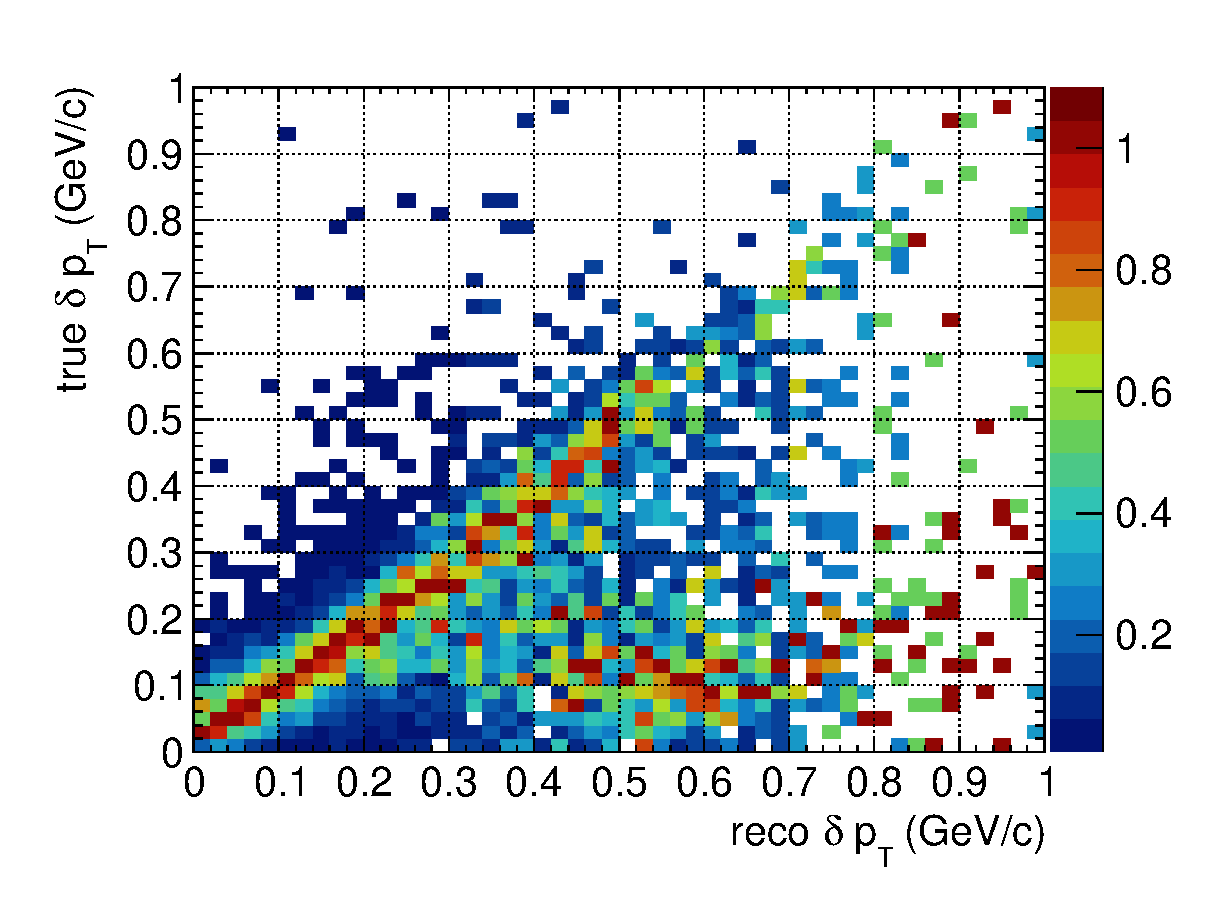
\includegraphics[width=\textwidth]{figures/perf/tki/dpt_colnor_resmat_al13.eps}
               \caption{$\dpt$ before ESC}
               \label{subfig:esc-dpt-bfesc}
          \end{subfigure}
          \begin{subfigure}[b]{\dbfigwid\textwidth}
               \centering
               \includegraphics[width=\textwidth]{figures/perf/tki/dpt_colnor_resmat_al14.eps}
               \caption{$\dpt$ after ESC}
               \label{subfig:esc-dpt-afesc}
          \end{subfigure}
          \\
          \begin{subfigure}[b]{\dbfigwid\textwidth}
               \centering
               \includegraphics[width=\textwidth]{figures/perf/tki/pn_colnor_resmat_al13.eps}
               \caption{$\pn$ before ESC}
               \label{subfig:esc-pn-bfesc}
          \end{subfigure}
          \begin{subfigure}[b]{\dbfigwid\textwidth}
               \centering
               \includegraphics[width=\textwidth]{figures/perf/tki/pn_colnor_resmat_al14.eps}
               \caption{$\pn$ after ESC}
               \label{subfig:esc-pn-afesc}
          \end{subfigure}
          \caption{TKI variables before and after ESC for the $\numucczpiop$ selection.}
          \label{fig:mc-tki-0pi-esc}
     \end{figure}

     The impact of the muon momentumn bias correction is better illurated with a resolution fit as shown in Fig.~\ref{fig:mc-tki-0pi-mubias}. 
     This correction has negligible impact on the angular vairables, but it helps to reduce bias in the momentum variables.
     As shown in Fig.~\ref{subfig:esc-dpt-bfmu} and Fig.~\ref{subfig:esc-dpt-afmu}, the $\dpt$ fitted mean improves from $0.92$ to $0.95$ after the muon bias correction.
     Similarly shown in Fig.~\ref{subfig:esc-pn-bfmu} and Fig.~\ref{subfig:esc-pn-afmu}, the $\pn$ fitted mean improves from $0.94$ to $1.01$.
     These reduction of bias can also be seen from the reduction of the over-estimated tails in the $\dpt$ and $\pn$ distributions.
     \begin{figure}
          \begin{subfigure}[b]{\dbfigwid\textwidth}
               \centering
               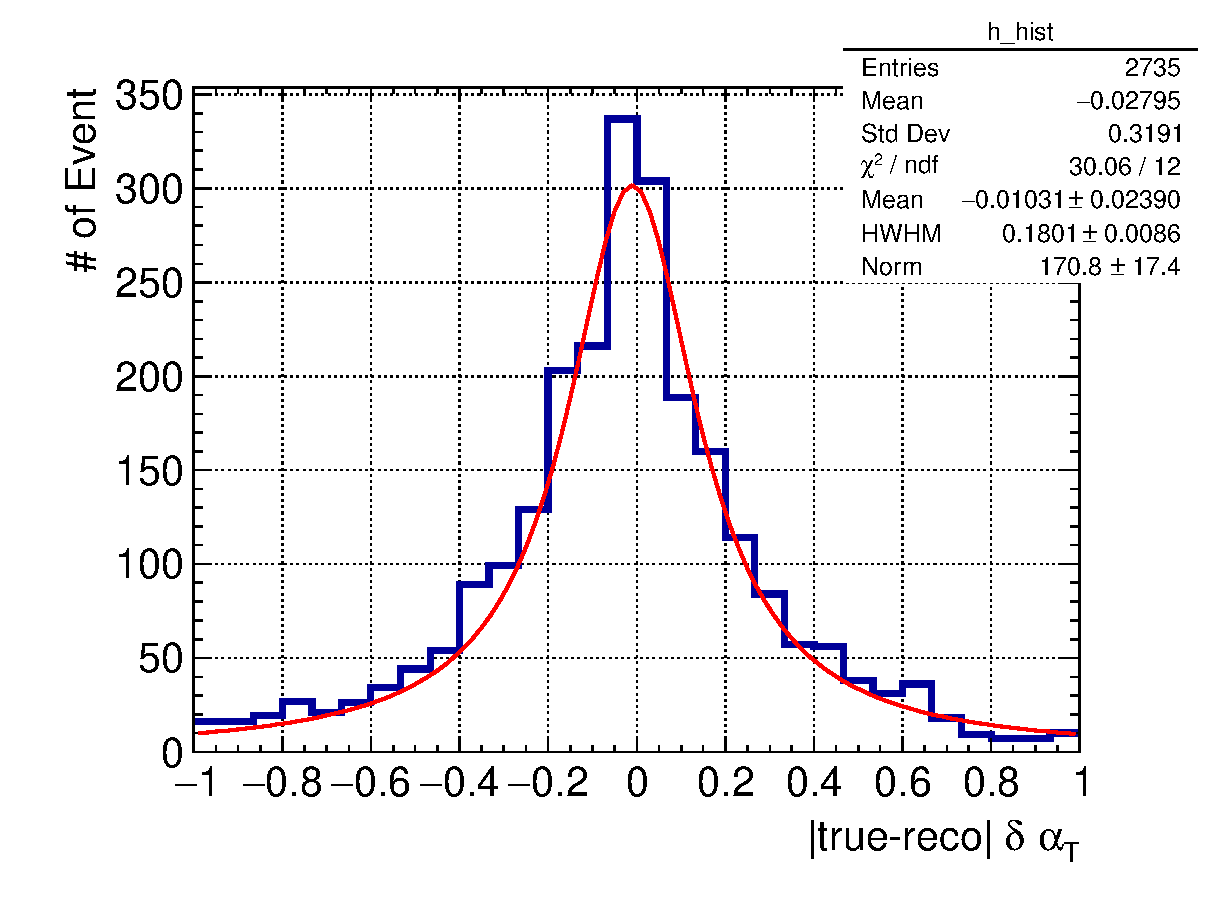
\includegraphics[width=\textwidth]{figures/perf/tki/dalphat_rat_hist_al14.eps}
               \caption{$\dat$ before muon bias correction}
               \label{subfig:esc-dalpha-bfmu}
          \end{subfigure}         
          \begin{subfigure}[b]{\dbfigwid\textwidth}
               \centering
               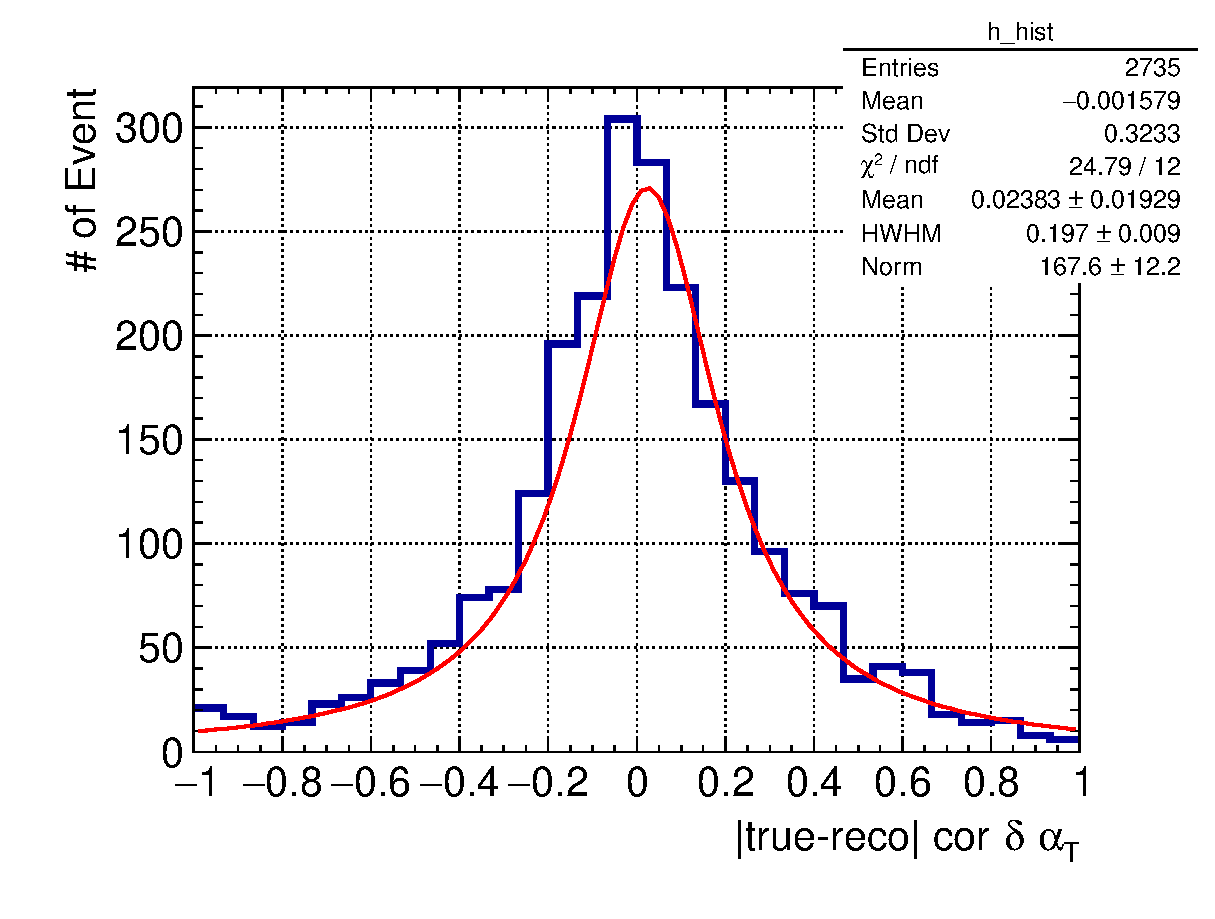
\includegraphics[width=\textwidth]{figures/perf/tki/cor_dalphat_rat_hist_al14.eps}
               \caption{$\dat$ after muon bias correction}
               \label{subfig:esc-dalpha-afmu}
          \end{subfigure}         
          \\
          \begin{subfigure}[b]{\dbfigwid\textwidth}
               \centering
               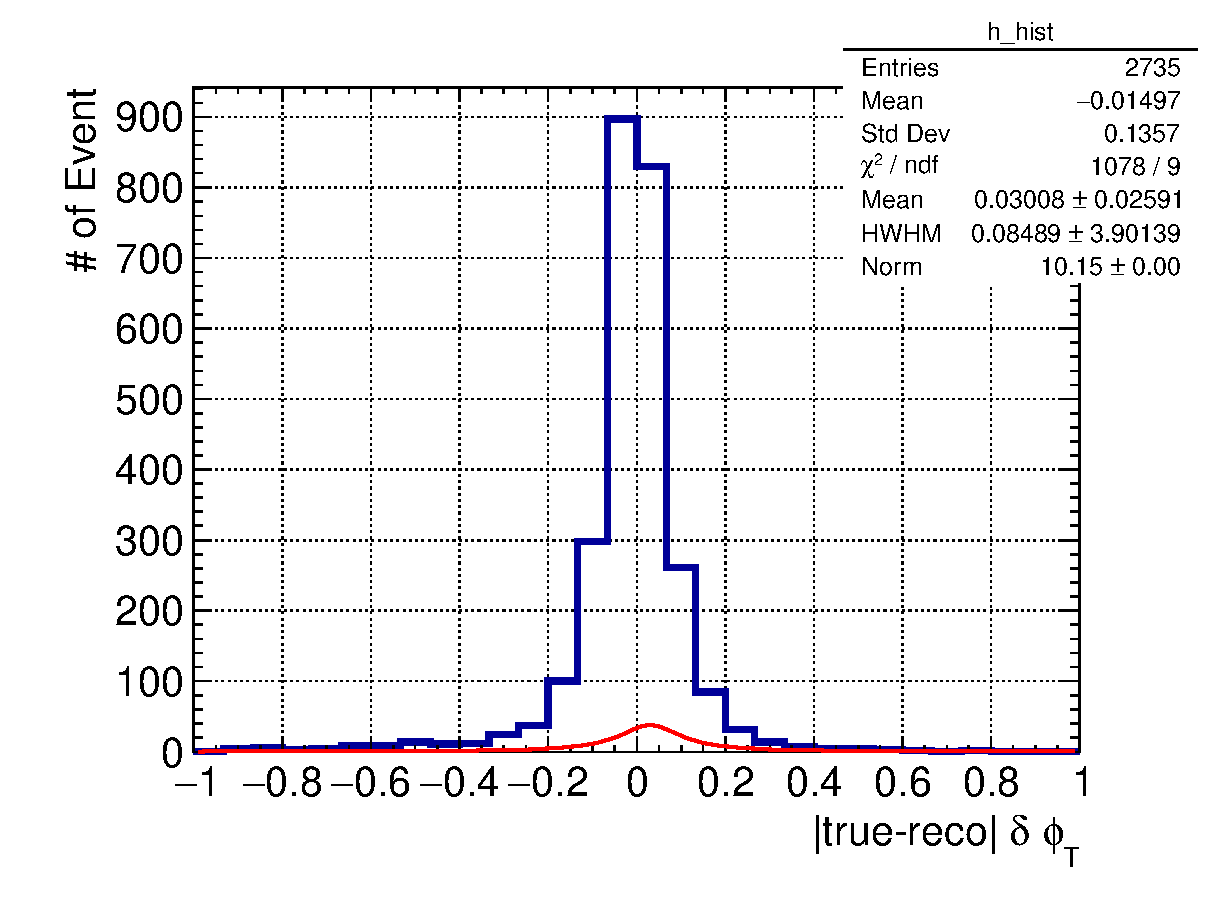
\includegraphics[width=\textwidth]{figures/perf/tki/dphit_rat_hist_al14.eps}
               \caption{$\dphit$ before muon bias correction (REPLOT NEEDED)}
               \label{subfig:esc-dphit-bfmu}
          \end{subfigure}
          \begin{subfigure}[b]{\dbfigwid\textwidth}
               \centering
               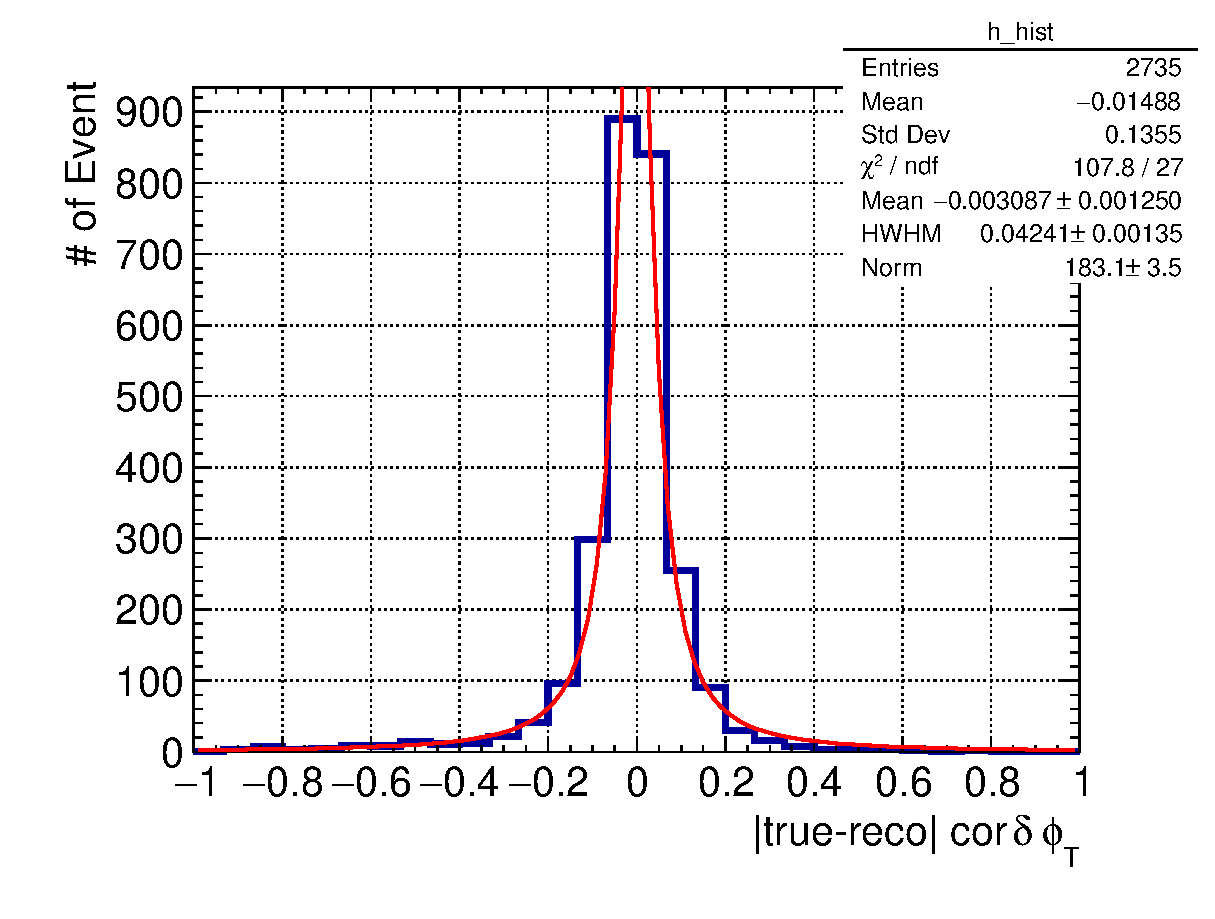
\includegraphics[width=\textwidth]{figures/perf/tki/cor_dphit_rat_hist_al14.eps}
               \caption{$\dphit$ after muon bias correction}
               \label{subfig:esc-dphit-afmu}
          \end{subfigure}
          \\
          \begin{subfigure}[b]{\dbfigwid\textwidth}
               \centering
               \includegraphics[width=\textwidth]{figures/perf/tki/dpt_rat_hist_al14.eps}
               \caption{$\dpt$ before muon bias correction}
               \label{subfig:esc-dpt-bfmu}
          \end{subfigure}
          \begin{subfigure}[b]{\dbfigwid\textwidth}
               \centering
               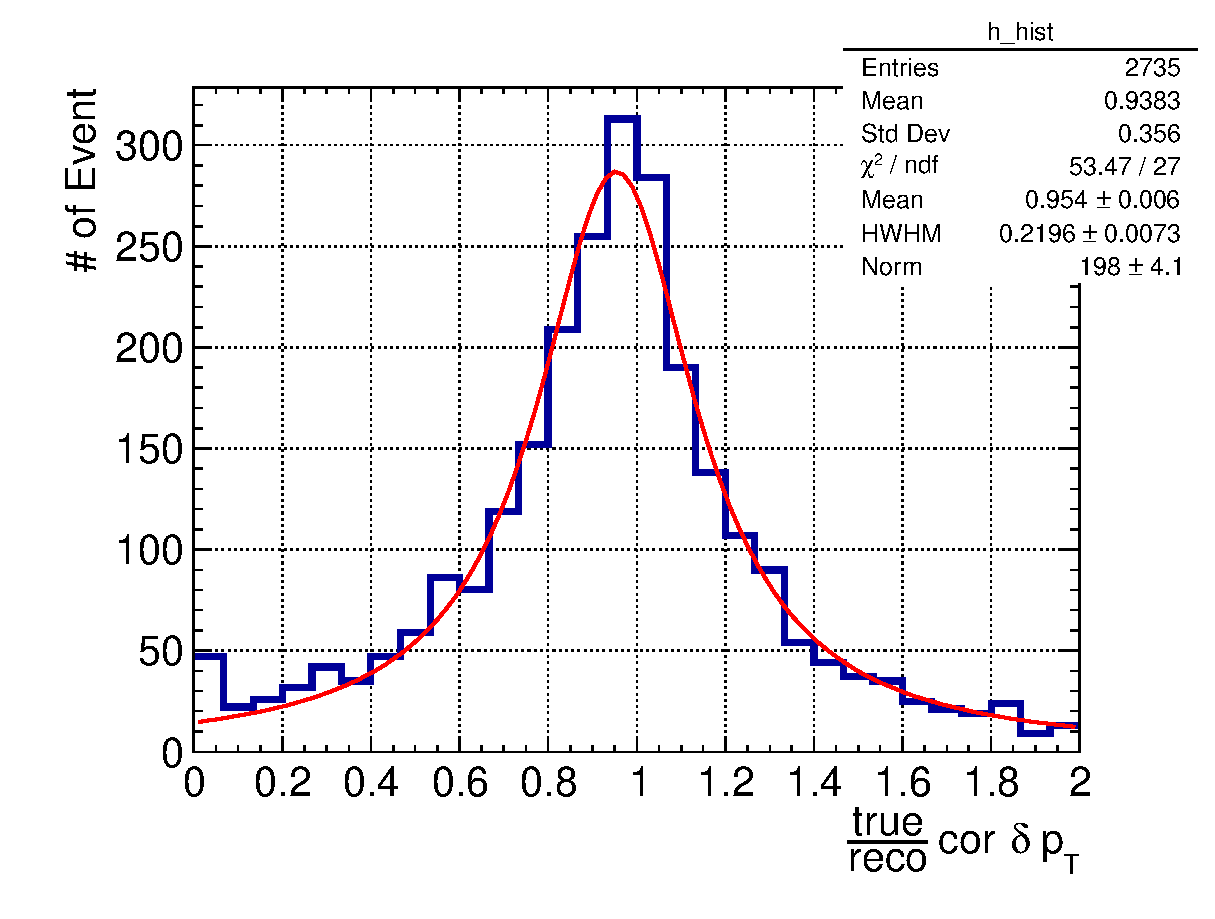
\includegraphics[width=\textwidth]{figures/perf/tki/cor_dpt_rat_hist_al14.eps}
               \caption{$\dpt$ after muon bias correction}
               \label{subfig:esc-dpt-afmu}
          \end{subfigure}
          \\
          \begin{subfigure}[b]{\dbfigwid\textwidth}
               \centering
               \includegraphics[width=\textwidth]{figures/perf/tki/pn_rat_hist_al14.eps}
               \caption{$\pn$ before muon bias correction}
               \label{subfig:esc-pn-bfmu}
          \end{subfigure}
          \begin{subfigure}[b]{\dbfigwid\textwidth}
               \centering
               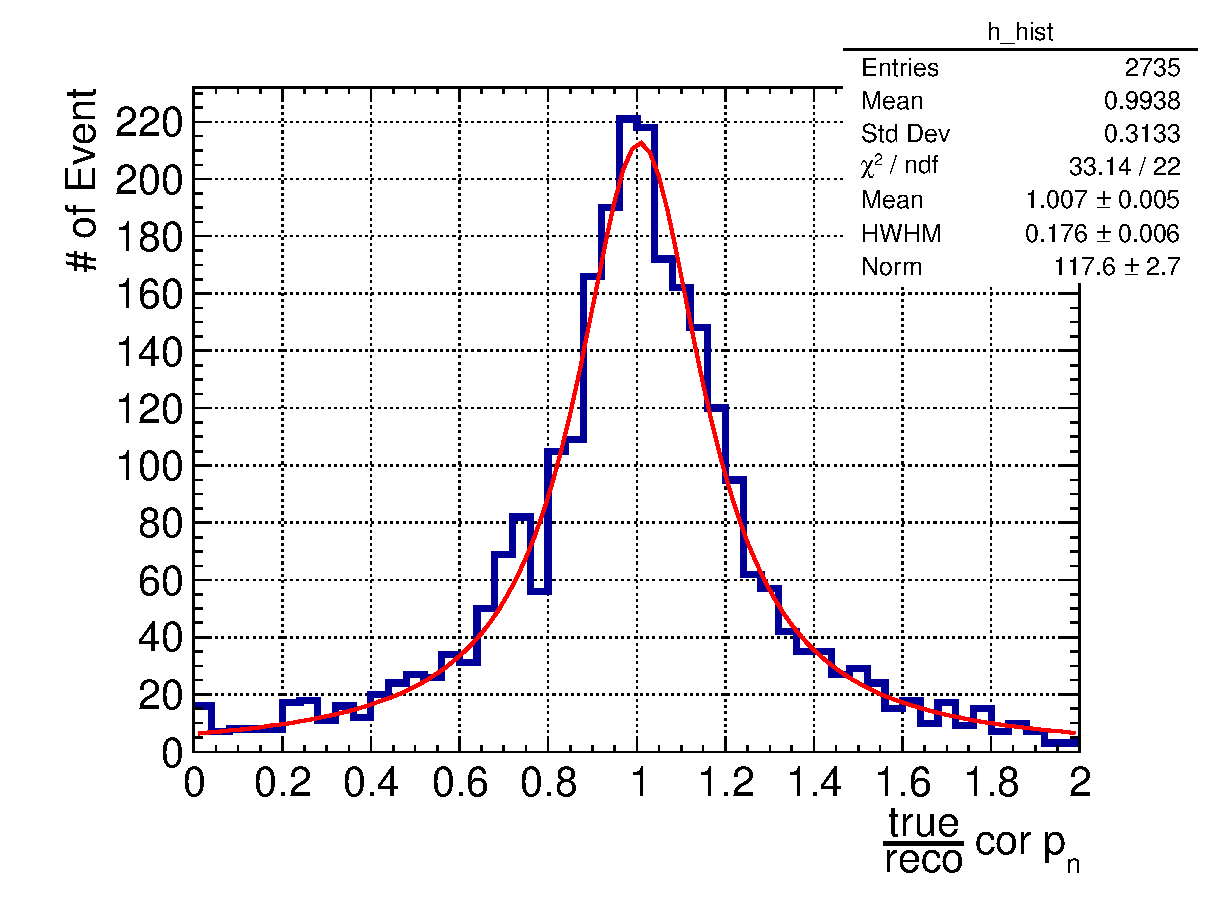
\includegraphics[width=\textwidth]{figures/perf/tki/cor_pn_rat_hist_al14.eps}
               \caption{$\pn$ after muon bias correction}
               \label{subfig:esc-pn-afmu}
          \end{subfigure}
          \caption{TKI variables before and after muon bias correction for the $\numucczpiop$ selection.}
          \label{fig:mc-tki-0pi-mubias}
     \end{figure}

     In Sec.~\ref{sec:sel-esc}, it has been shown that the ESC technique has improved the proton momentum reconstruction resolution while reducing the efficiency by about $60~\%$.
     The result shown in this section further demonstrates the necessity of the ESC technique for the TKI measurements.
     With the ESC technique, the T2K upgraded ND possess the potential of high resolution TKI measurements with minimal bias.
     Recently, there has been an update on the TKI measurement at the pre-upgrade ND280 data using an improved reconstruction algorithm.
     This leads to a standard deviation of approximately $27\%$ for the $\pn$ reconstruction resolution. 
     The resolution of $30\%$ for the TPC-$\mu$ sub-sample is comparable to this improvement, while the resolution of about $17\%$ for the SFGD-$\mu$ sub-sample is significantly better.
     There is still room for improvement for the upgrade measurement as the global reconstruction matures.    

     \subsection{$\numuccopiop$ selection}
     \label{sec:mc-tki-1pi}
     The $numuccopiop$ selection uses the pion trackless reconstruction technique as elaborated in Sec.~\ref{sec:sel-tl} for the $\numuccopi$-TL selection.
     Additionally, it requires the reconstruction of one ESC proton.
     Hence, this sample uses both novel techniques in Chapter~\ref{ch:sel}, showcasing the potential of the upgraded ND280 detector in hadronic measurement.

     The TKI variables for the $\numuccopiop$ selection are shown in Fig.~\ref{fig:mc-tki-1pi}.
     \begin{figure}
          \begin{subfigure}[b]{\dbfigwid\textwidth}
               \centering
               \includegraphics[width=\textwidth]{figures/perf/tki/SFGpTPCmu_dalphat_rat_hist_al14.eps}
               \caption{$\dat$}
               \label{subfig:1pi-dalpha}
          \end{subfigure}         
          \begin{subfigure}[b]{\dbfigwid\textwidth}
               \centering
               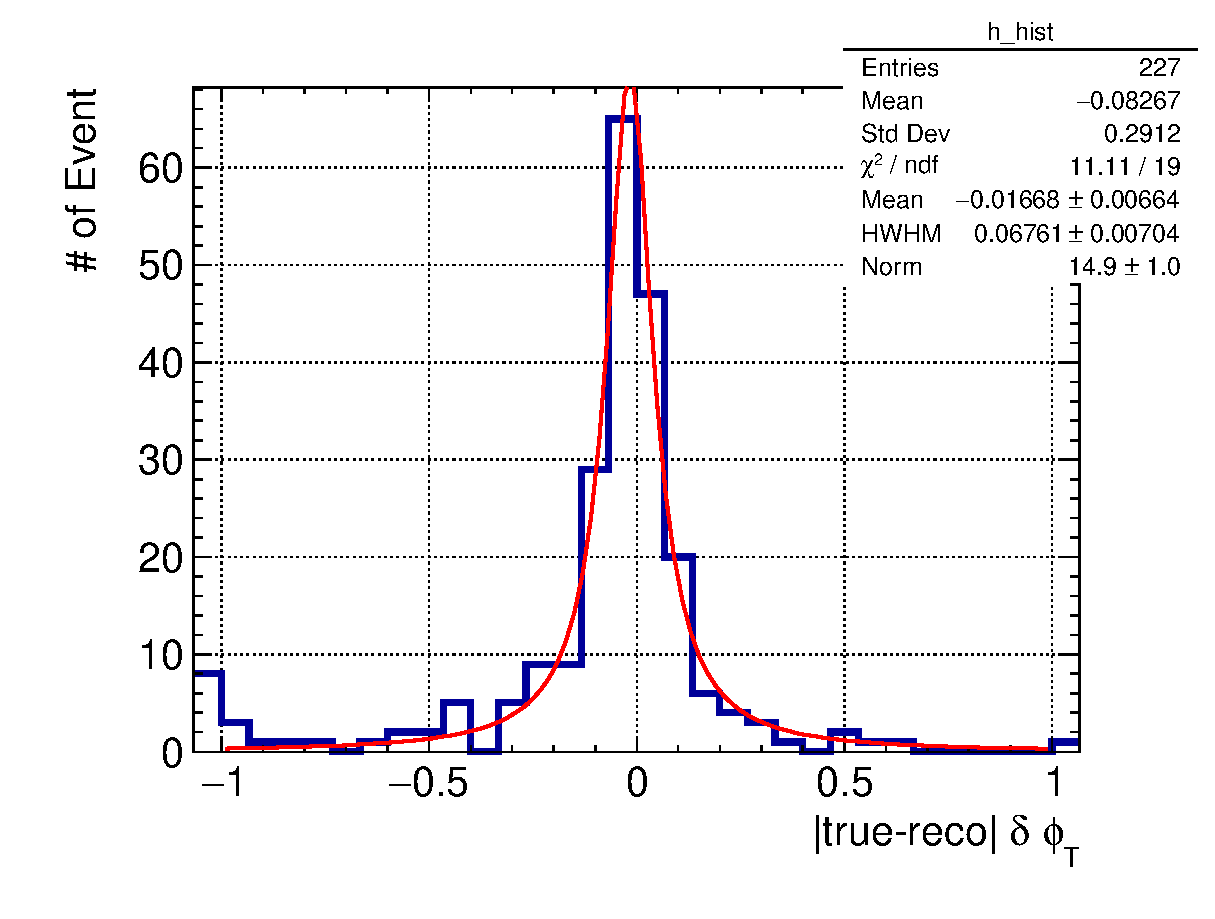
\includegraphics[width=\textwidth]{figures/perf/tki/SFGpTPCmu_dphit_rat_hist_al14.eps}
               \caption{$\dphit$}
               \label{subfig:1pi-dphit}
          \end{subfigure}
          \\
          \begin{subfigure}[b]{\dbfigwid\textwidth}
               \centering
               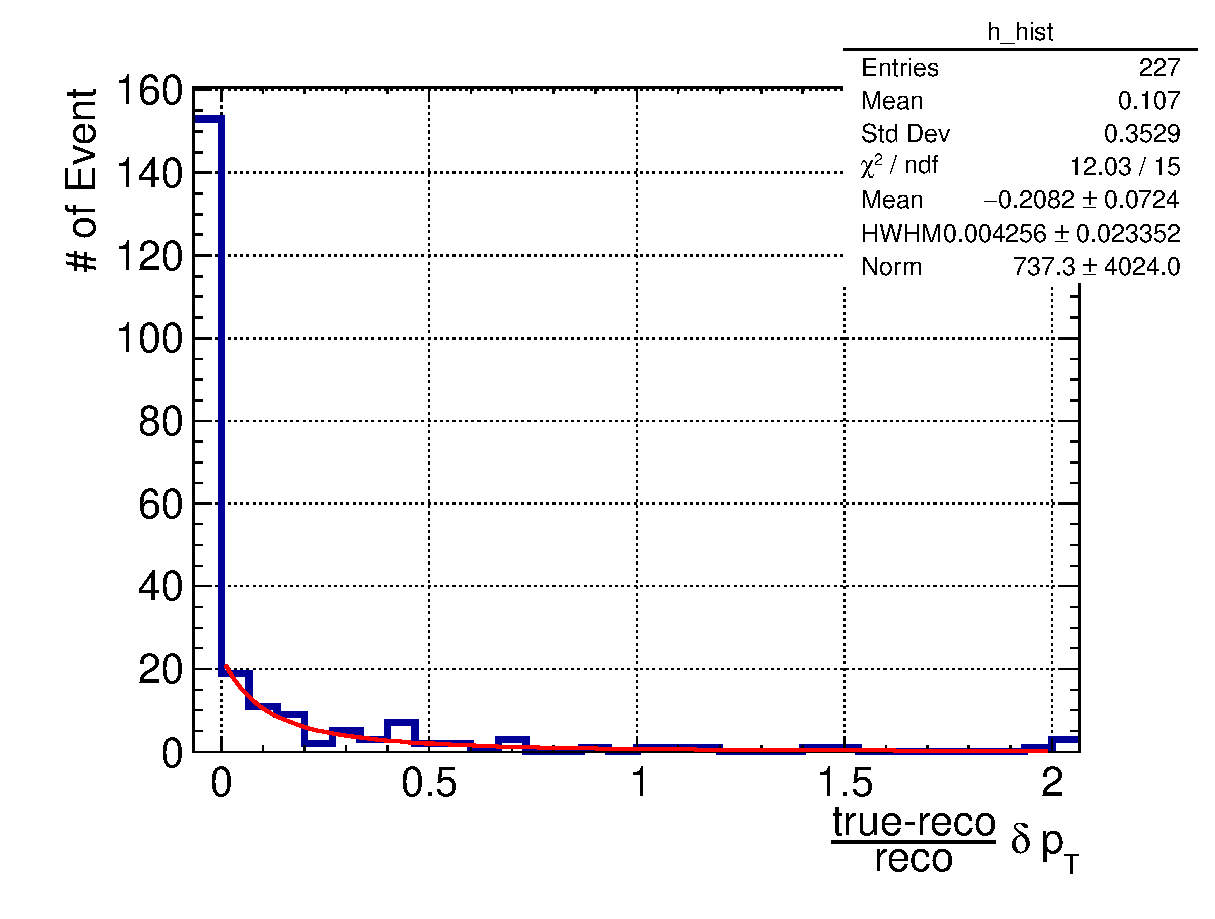
\includegraphics[width=\textwidth]{figures/perf/tki/SFGpTPCmu_dpt_rat_hist_al14.eps}
               \caption{$\dpt$}
               \label{subfig:1pi-dpt}
          \end{subfigure}
          \begin{subfigure}[b]{\dbfigwid\textwidth}
               \centering
               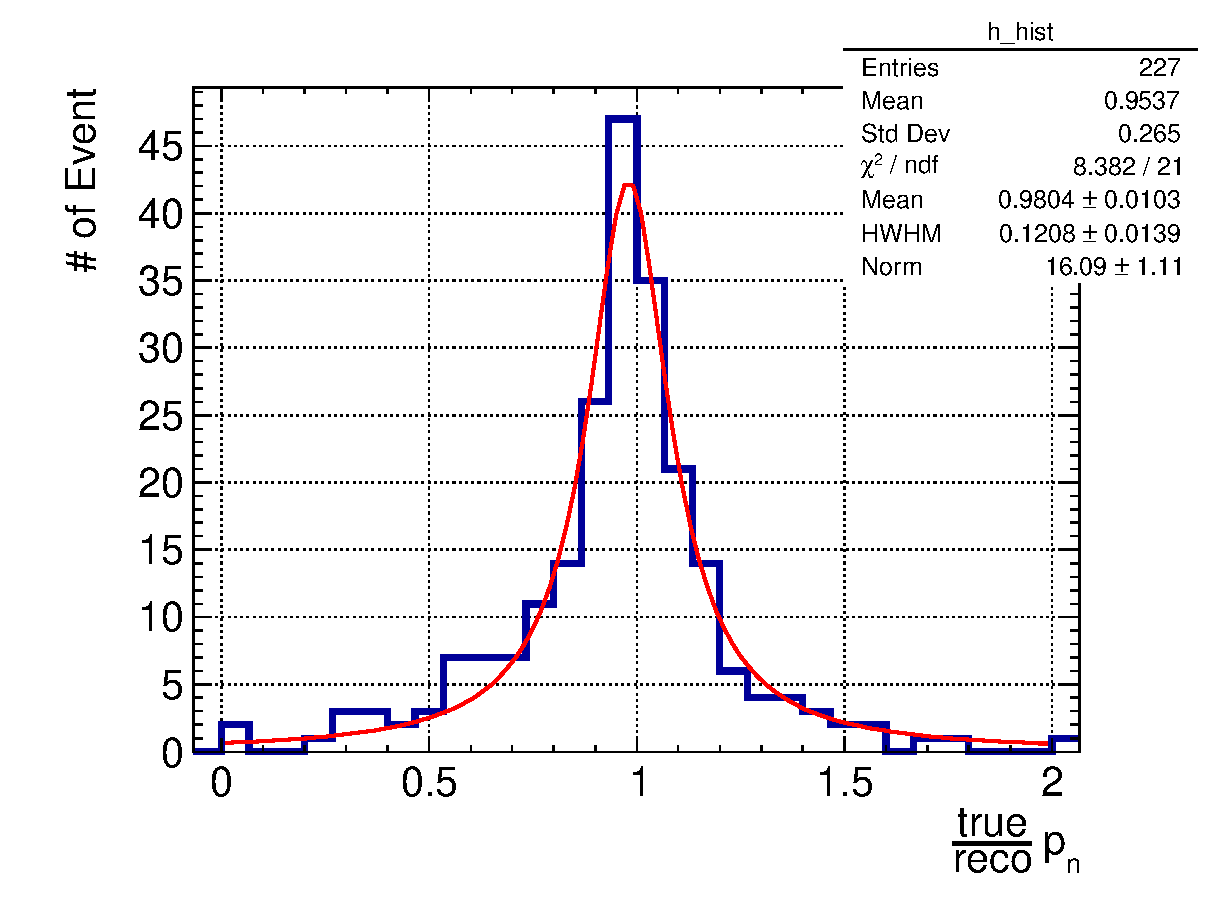
\includegraphics[width=\textwidth]{figures/perf/tki/SFGpTPCmu_pn_rat_hist_al14.eps}
               \caption{$\pn$}
               \label{subfig:1pi-pn}
          \end{subfigure}
          \caption{TKI variables for the $\numuccopiop$ selection.}
          \label{fig:mc-tki-1pi}
     \end{figure}
     

     In comparison to the projected resolution of the $\dptt$ measurement using the pre-upgrade ND280 in Ref.~\cite{lu:2015hea}, Fig.~\ref{1pi-tki-dptt} shows a $60\%$ decrease in the $\dptt$ width, 

     In additional to the single transverse variables presented above, the $\numuccopiop$ sample can also be used to measure the double transverse variable, $\dptt$, the net momentum transverse to both the neutrino momentum and the muon momentum,
     The $\dptt$ resolution is shown in Fig.~\ref{fig:1pi-tki-dptt}.
     Without FSI, $\dptt$ should be $0$. This special property can be exploited to select $\nu$-H events amidst $\nu$-C events as suggested in Ref.~\cite{dpttpaper}. 
     Hence, the main figure of merit for $\dptt$ measurement is the width of its distribution for $\nu$-H events, where the hydrogen events are picked by an additional check on the MC truth information.
     As shown in Fig.~\ref{fig:1pi-tki-dptt}, the fitted half width is about $12~\mevc$, which is significantly improved compared to $21~\mevc$, the pre-upgrade ND280 result~\cite{lu:2015hea}, suggesting a greater potential to apply it for a hydrogen sample selection, which will be discussed at the end of this chapter in Sec.~\ref{sec:mc-hydrogen}.

     \begin{figure}[!htb] 
          \centering 		
          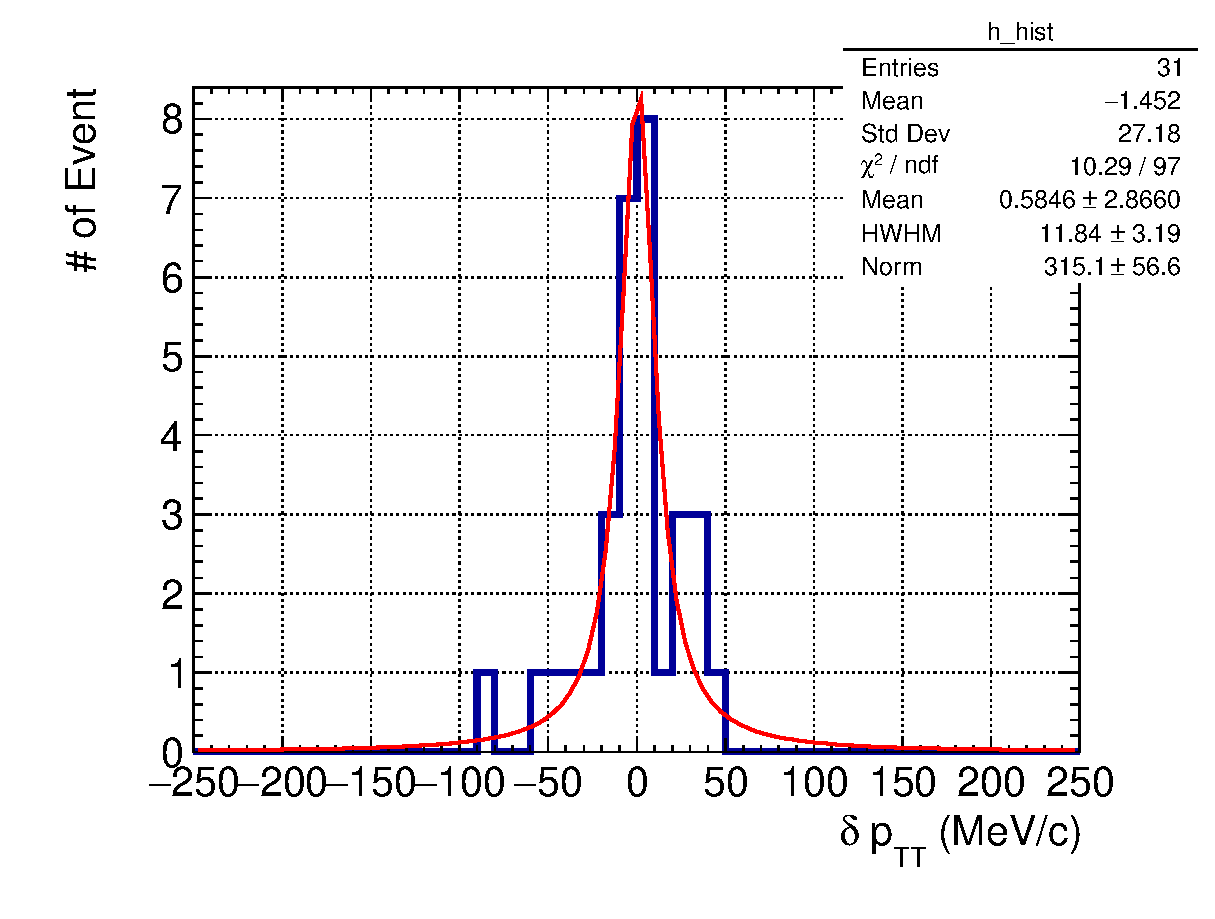
\includegraphics[width=\sgfigwid\textwidth]{figures/perf/tki/SFGpTPCmu_dptt_hist_al15_H_bin100_range500_Lfit.eps}
          \caption{\label{fig:1pi-tki-dptt} $\dptt$ distribution for $\nu$-H events.} 
     \end{figure}


\section{COM}
\label{sec:mc-com}
When a neutrino has sufficient energy, it can excite a nucleon into a resonance state, for example the $\deltapp$. 
This process is referred to as a resonance (RES) interaction.
Since $\deltapp$ is one of the most commonly observed resonances in neutrino experiments, this work focuses on it as an example.
Nevertheless, the concept presented here is equally applicable to other resonances, and the methodology can be easily generalized.

The resonance decays rapidly, before leaving the nucleus, via the process
\begin{equation}
     \deltapp \rightarrow \pip + \p.
\end{equation}
In the $\deltapp$ rest frame, as illustrated on the top left in Fig.~\ref{fig:COM-diagram}, the kinematics of this two-body decay are well-defined and the proton and pion are emitted back-to-back.
The pion decay angle, $\thetapidel$, is defined as the angle between $\vecppirest$ and the $x$-axis, which is taken to align with $\vecpdel$, the momentum of $\deltapp$ in the lab frame. 
$\thetapidel$ is a resonance property that follows an underlying distribution defined by various models~\cite{Rein:1987cb,Kabirnezhad:2017jmf,Kabirnezhad:2020wtp,Kabirnezhad:2022znc}.

\begin{figure}[ht!]
\centering
\includegraphics[width=\linewidth]{figures/COM/COM-diagram.pdf}
\caption{Schematic illustration of the COM angle. Without FSI, $\vecpsum=\vecpdel$ and the lab frame and the $\deltapp$ rest frame can be transformed into each other by $\vecpdel$. With FSI, $\vecpsum \neq \vecpdel$, the $\deltapp$ rest frame is not accessible, but the lab frame can be boosted into the COM frame using $\vecpsum$. Hence, the major difference of the COM frame from the $\deltapp$ rest frame is caused by FSI.}
\label{fig:COM-diagram}
\end{figure}

The kinematics in the lab frame are related to those in the $\deltapp$ rest frame by a boost with $\vecpdel$, as depicted on the top right of Fig.~\ref{fig:COM-diagram}. 
Without FSI, $\vecpdel$ equals the sum of $\vecpp$ and $\vecppi$.
However, the target materials of modern day detectors are mainly comprised of nucleus with multiple nucleons and FSI alters the kinematics of the hadrons considerably, as illustrated by the dotted arrows in the bottom right of Fig.~\ref{fig:COM-diagram}.

The altered momenta, $\vecppp$ and $\vecppip$, are the ones measured by detectors. 
Their sum generally differs from $\vecpdel$.
Thus, the $\deltapp$ rest frame with its simple kinematic relations becomes inaccessible.
Nevertheless, the system can be boosted to the proton-pion COM frame using $\vecpsum$, as depicted in the bottom left of Fig.~\ref{fig:COM-diagram}, where the $x^{\prime}$-axis is taken to align with the $\vecpsum$ direction in the lab frame.
Similarly, a pion decay angle, $\thetacom$, can be defined between, $\vecppicom$, the pion momentum in the COM frame, and the $x^{\prime}$-axis.
Due to FSI, $\thetacom$ typically differs from $\thetapidel$. 

The COM frame coincides with the $\deltapp$ rest frame only in the absence of FSI.
Thus, the strength of FSI dictates the deviation of $\thetacom$ from $\thetapidel$. 
In practice, the measured $\thetacom$ serves as a probe for studying FSI. 
$\thetapidel$, being a rest-frame property of $\deltapp$, is independent of the resonance's momentum, neutrino energy, and IS.
In neutrino event generators, $\thetacom$ deviates from $\thetapidel$ only due to FSI, which is independent of neutrino energy and IS.
Therefore, $\thetacom$ retains these important independencies.
As different resonances could have different decay properties, $\thetaR$, the similarly defined pion decay angle of a higher resonance, $R$, generally differs from $\thetapidel$. 
Hence, $\thetacom$, a superposition of $\thetapidel$ and all possible $\thetaR$, will deviate from $\thetapidel$, when more resonances become energetically possible with an increase in neutrino energy. 
This deviation will be further elaborated in the Sec.~\ref{sec:dis}.

Moreover, the total energy in the COM frame, $\ecom$, will be equal to the mass of the resonance in the absence of FSI.
Cutting on events with total energy far from the rest mass peak of the resonance will select events with minimal FSI effects, such as the $\nu$-H events. 
The application of $\ecom$ for hydrogen event selection will be discussed in Sec.~\ref{sec:mc-hydrogen}.

Up to this point, the discussion of resonance decay has been entirely general and can thus be applied to and validated by various experiments, including hadron scattering measurements. 
However, there are features specific to neutrino experiments. 
First, the resonance is generated through neutrino-nucleon interactions, which involve both vector and axial currents. 
Second, the interaction occurs within the nuclear medium. 
This work focuses on the latter, with the application of COM variables to the former reserved for future research.

While the COM angle may appear conceptually similar to the reconstructed Adler angle, $\thetaadt$, in neutrino experiments~\cite{Sanchez:2015yvw}, there are significant differences. 
Notably, the COM frame is reconstructed exclusively from hadronic kinematics, whereas the reconstructed Adler frame relies on leptonic kinematics and assumes stationary nucleons. 
Consequently, the reconstruction of the Adler frame is implicitly influenced by IS effects, whereas the COM frame's hadronic variables are impacted by final state interactions (FSI). 
Therefore, $\thetaadt$, being a hadronic variable in the Adler frame, is influenced by both IS and FSI. 
Additionally, the necessity of reconstructing the neutrino energy renders $\thetaadt$ sensitive to neutrino flux uncertainties, which are among the largest systematic uncertainties in neutrino measurements~\cite{T2K:2019yqu,T2K:2021naz,MicroBooNECollaboration:2024gvg,NOvA:2023uxq,MINERvA:2022djk}.


     \subsection{Analysis result}
     \label{sec:com-ana}
     In the absence of existing measurements of the COM angle, MC studies were conducted to evaluate its potential advantages.
     MC samples were generated using \genie \cite{Andreopoulos:2009rq, GENIE:2021npt} for T2K beam and target. 
     Several \genie tunes were compared, with the model details for each tune summarized in Table~\ref{tab:genie-tunes}. 
     Each sample consists of $600,000$ muon neutrino events, and a selection of charge current single pion and single proton ($\numuccopiop$) events was used to generate the plots.

     \begin{table}[h]
     \centering
     \begin{tabular}{c|c|c|c|c|c}
          CMC                  &  IS  &  QE                & 2p2h         & RES & FSI\\
          \hline
          G18\_01a\_02\_11b    &  RFG         &   LS               & Dytman       & RS  & hA\\
          G18\_02a\_02\_11b    &  RFG         &   LS               & Dytman       & BS  & hA\\
          G18\_10a\_02\_11b\footnote{The \genie default uses local Fermi gas instead.}    
                              &  CFG         &  Valencia          & Nieves       & BS  & hA\\
          G18\_10b\_02\_11b    &  LFG         &  Valencia          & Nieves       & BS  & hN\\
          G24\_20i\_00\_000    &  SF-CFG      &  Valencia          & SuSAv2       & BS  & hA\\
          G24\_20i\_06\_22c    &  SF-CFG      &  Valencia          & SuSAv2       & BS  & hA(tuned)\\
     \end{tabular}
     \caption{The four nuclear IS models are relativistic Fermi gas (RFG), local Fermi gas (LFG), correlated Fermi gas (CFG), spectral-function-like CFG (SF-CFG)~\cite{sfcfg-talk,sfcfg-GitHubCommit,GENIE:2021npt}. 
     The respective cross-section models are: 1) Quasielastic (QE) - Llewellyn-Smith (LS)~\cite{LlewellynSmith:1971uhs} and Valencia~\cite{Nieves:2004wx}; 2) 2p2h - Dytman~\cite{genie:2p2h-dytman}, Nieves~\cite{Nieves:2011pp} and SuSAv2~\cite{Gonzalez-Jimenez:2014eqa}; 3) RES - Rein-Sehgal~\cite{Rein:1980wg} and Berger-Sehgal~\cite{Berger:2007rq}. 
     The FSI models are the built-in \genie models~\cite{Andreopoulos:2015wxa}, INTRANUKE hA and hN. Note that in \texttt{G24\_20i\_06\_22c}~\cite{GENIE:2024ufm}, the hA model has been tuned using TKI data, resulting in parameters that differ from the default hA.}
     \label{tab:genie-tunes}
     \end{table}


     \begin{figure}[ht!]
     \centering
     \begin{subfigure}[ht!]{\dbfigwid\textwidth}
          \centering
          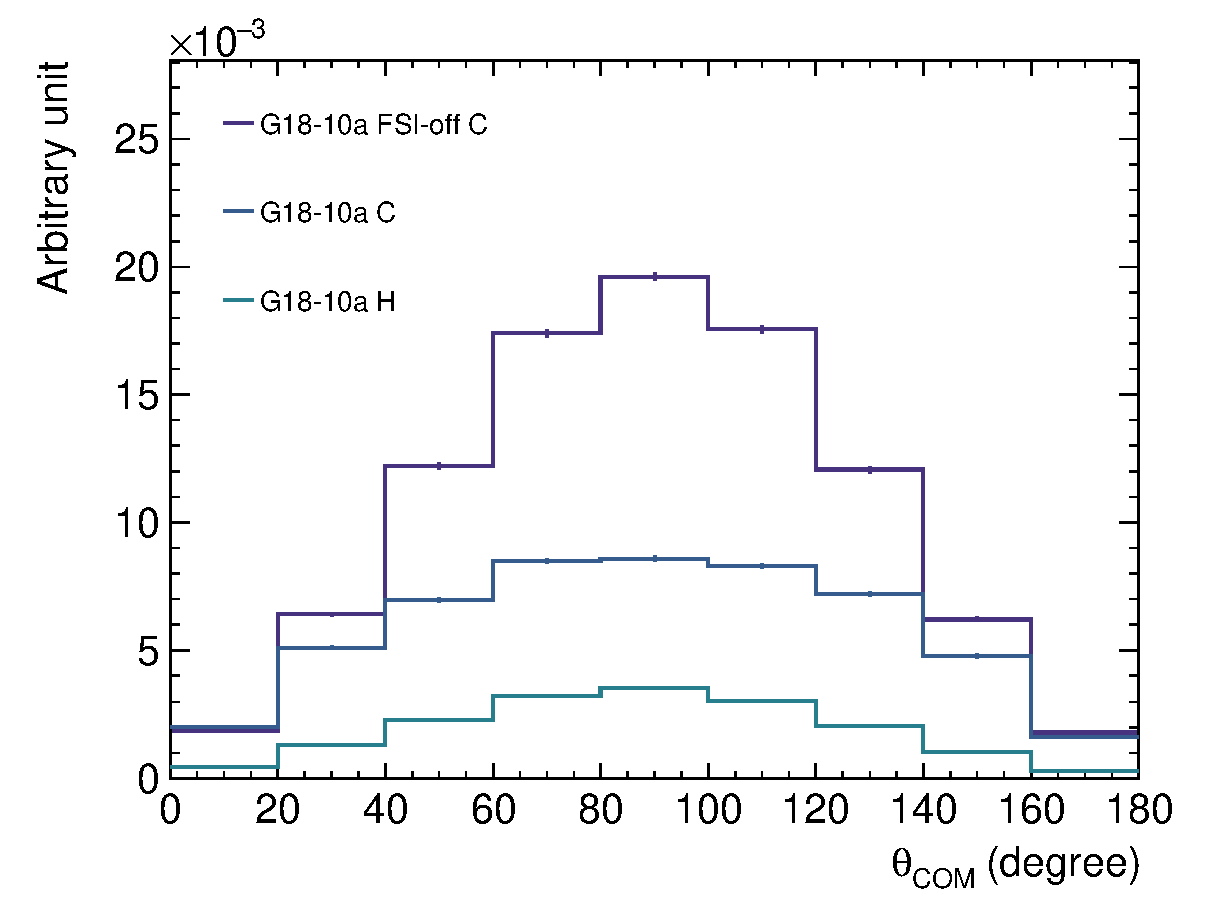
\includegraphics[width=\textwidth]{figures/COM/xnorm-CH_da_tan.eps} \\
          \caption{Cross-section normalized comparisons with FSI on/off for carbon and hydrogen with \texttt{G18\_10a\_02\_11b}.}
          \label{subfig:fsi-comp-chof}
     \end{subfigure}
     \begin{subfigure}[ht!]{\dbfigwid\textwidth}
          \centering
          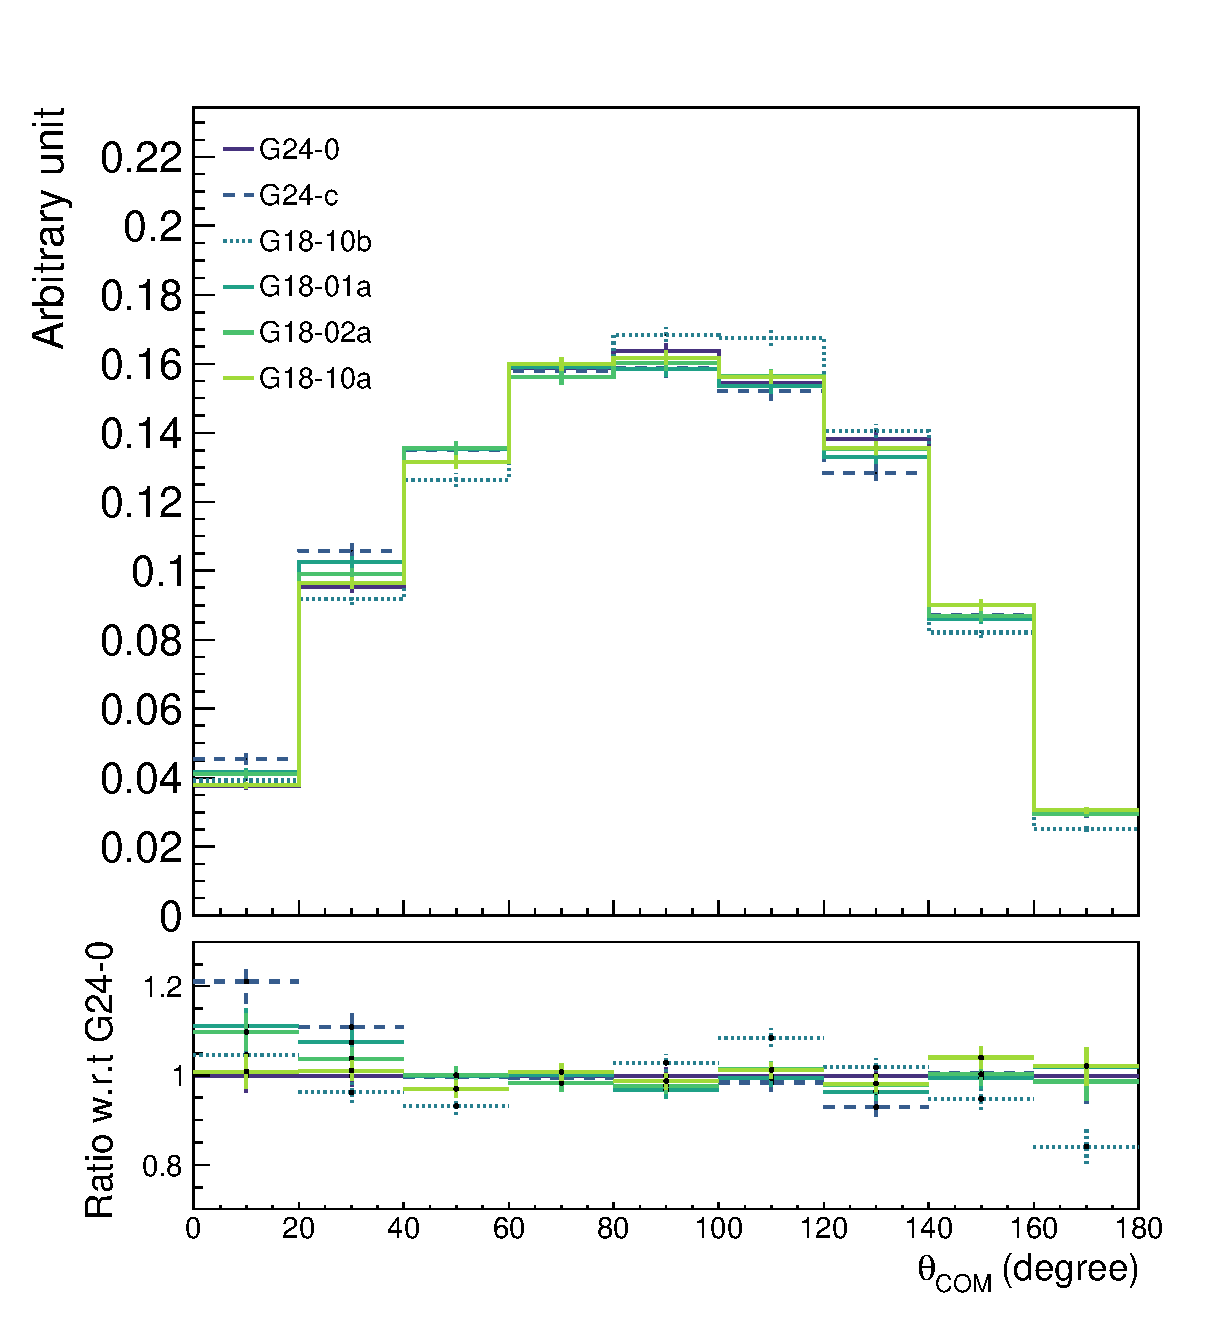
\includegraphics[width=\textwidth]{figures/COM/anorm-mod-ratio-_da_tan.eps}
          \caption{Area normalized comparisons for different tunes with FSI on for carbon. }
          \label{subfig:fsi-comp-gt}
     \end{subfigure}
     \caption{\blue{$\thetacom$ distribution comparisons using T2K flux on different nuclei and with multiple \genie configuations.} }
     \label{fig:fsi-comp}
     \end{figure}

     As illustrated in Fig.~\ref{fig:fsi-comp} (a), enabling or disabling FSI has a significant effect on the $\thetacom$ cross-section as expected.
     More critically, Fig.~\ref{fig:fsi-comp} (b) shows that changing the underlying FSI model from hA (10a) to hN (10b) or from hA (10a) to hA (tuned, G24-c) results in a noticeable variation in the $\thetacom$ cross-section. 
     In contrast, although numerous combinations of IS, QE, 2p2h, and RES models were tested, configurations using the hA FSI model produced nearly identical cross-sections.
     This demonstrates the potential of $\thetacom$ to distinguish between different FSI models, independent of many other factors.


     To further examine the independence from IS of $\thetacom$, the cross-section shape of $\nu$-C (with FSI on and off) is compared to that of $\nu$-H. 
     The $\nu$-H interaction is free from any nuclear effects, while $\nu$-C without FSI reflects the impact of IS, including carbon removal energy and Fermi motion. 
     When FSI is on, the full nuclear effects—both IS and FSI—are present. 
     Fig.~\ref{subfig:ch-comp-com-cc1pi1p} shows that FSI has a substantial impact on the cross-section shape, as expected. 
     The near overlap of the $\nu$-H and $\nu$-C (FSI-off) curves provides strong evidence for the proposed independence of $\thetacom$ from IS effects.

     \begin{figure}
     \centering
     \begin{subfigure}[ht!]{\dbfigwid\textwidth}
          \centering
          \includegraphics[width=\textwidth]{figures/COM/anorm-CH_da_tan.eps}     
          \caption{$\thetacom$ - general $\numuccopiop$.}
          \label{subfig:ch-comp-com-cc1pi1p}
     \end{subfigure}
     \begin{subfigure}[ht!]{\dbfigwid\textwidth}
          \centering
          \includegraphics[width=\textwidth]{figures/COM/anorm-CH_adt.eps}        
          \caption{$\thetaadt$ - general $\numuccopiop$.}
          \label{subfig:ch-comp-adt-cc1pi1p}
     \end{subfigure} 
     \caption{\blue{Area normalized comparisons for FSI on/off for carbon and hydrogen with \texttt{G18\_10a\_02\_11b} between $\thetacom$ and $\thetaadt$ using T2K flux and target.}  with the bottom row has a more stringent selection to restrict the resonance to be $\deltapp$.}
     \label{fig:ch-comp}
     \end{figure}

     Although $\thetacom$ is conceptually similar to the reconstructed Adler angle, $\thetaadt$, the latter is additionally influenced by IS effects. 
     However, Fig.~\ref{subfig:ch-comp-adt-cc1pi1p}  suggests that the $\nu$-H and $\nu$-C (FSI-off) curves remain nearly as close as in Fig.~\ref{subfig:ch-comp-com-cc1pi1p}. 
     When a stricter selection is made to select only events involving $\deltapp$ as shown in Fig.~\ref{fig:ch-comp-dpp} in Appendix, the small difference in $\thetacom$ reduces further while the two curves deviate slightly more in $\thetaadt$. 
     This suggests that in the absence of FSI, $\thetacom$ could be a better construction of $\theta$ than $\thetaadt$. 

     Nevertheless, the small difference between the two curves for $\thetaadt$ indicates that despite IS dependence, IS does not significantly distort the shape of $\thetaadt$ appreciably.
     This observation could challenge the claimed IS independence of $\thetacom$, as it might be due to the relatively minor influence of IS. 
     To further examine this, a stress test was conducted by varying the removal energy of carbon across a wide range, even to unphysical levels, to assess its effect on the shapes of $\thetacom$ and $\thetaadt$. 
     The results are presented in Fig.~\ref{fig:ermc-comp}.

     \begin{figure}[ht!]
     \centering
     \begin{subfigure}[ht!]{\dbfigwid\textwidth}
          \centering
          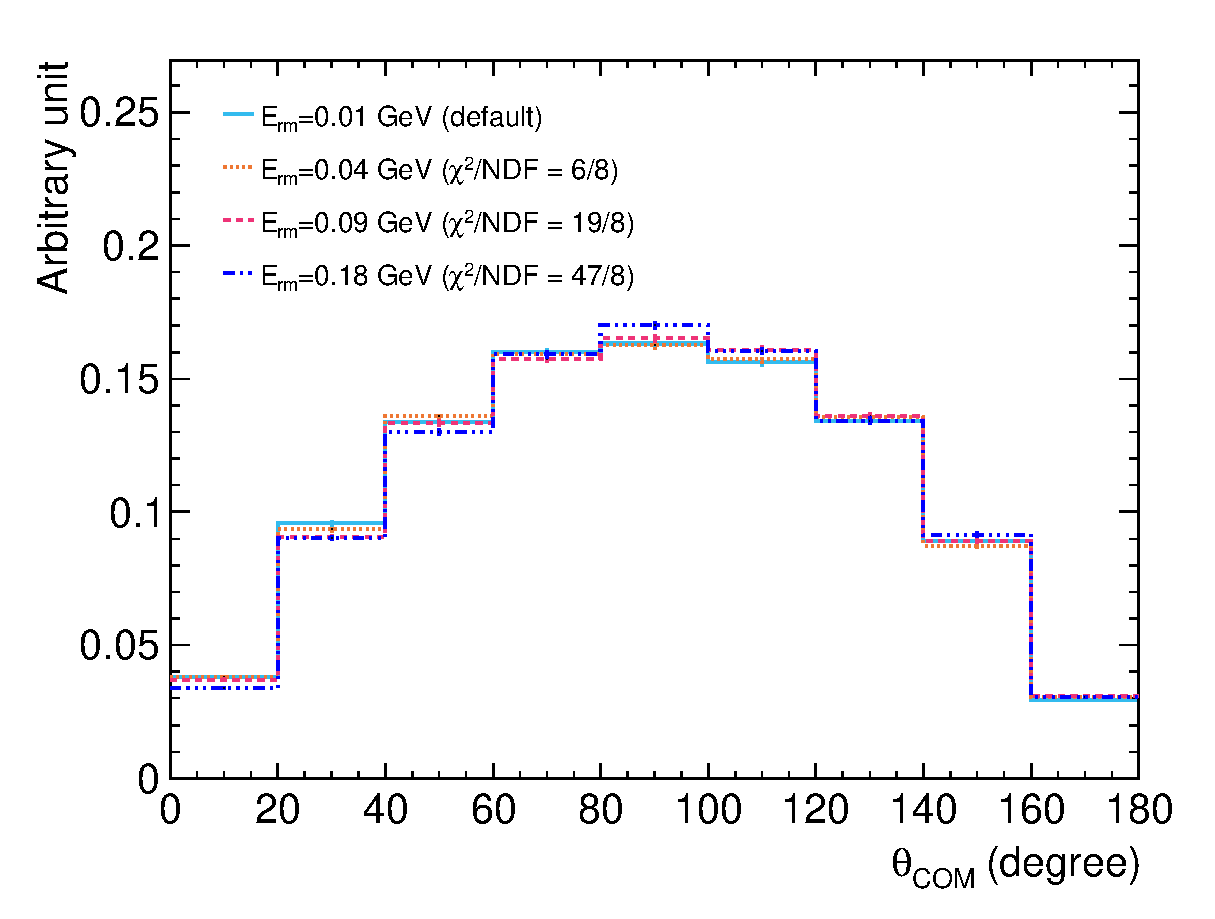
\includegraphics[width=\textwidth]{figures/COM/anorm-nuc_da_tan.eps}
          \caption{$\thetacom$}
          \label{subfig:ermc-comp-com}
     \end{subfigure}
     \begin{subfigure}[ht!]{\dbfigwid\textwidth}
          \centering
          \includegraphics[width=\textwidth]{figures/COM/anorm-nuc_adt.eps}
          \caption{$\thetaadt$}
          \label{subfig:ermc-comp-adt}
     \end{subfigure}
          
     \caption{Area normalized comparisons for different removal energies, $E_{\textrm{rm}}$, with T2K flux.}
     \label{fig:ermc-comp}
     \end{figure}

     As seen in Fig.~\ref{fig:ermc-comp}, variations in the removal energy ($E_{\textrm{rm}}$) do not affect $\thetacom$ at all. 
     In contrast, the $\thetaadt$ peak exhibits a noticeable shift, along with a gradual change in its shape.
     These results confirm that $\thetacom$ is independent of IS effects, while $\thetaadt$ exhibits IS dependence, as predicted.

     Another important feature of $\thetacom$ is its independence from neutrino energy. 
     Fig.~\ref{fig:enu-comp} illustrates this behavior. 
     The $\thetacom$ distribution shapes remain largely consistent for $\enu$ values between $0.5~\gev$ and $2.0~\gev$ across most angles.
     However, deviations become more pronounced at smaller angles. 
     As $\enu$ increases to $5\gev$, a noticeable rise is observed in the small-angle region, likely due to the onset of a higher doubly positive resonance. 
     If the analysis is limited to $\deltapp$ as in Fig.~\ref{fig:enu-comp}(b), it is encouraging to observe that the different curves converge, confirming the independence of $\thetacom$ from $\enu$.

     \begin{figure}[ht!]
     \centering
     \begin{subfigure}[ht!]{\dbfigwid\textwidth}
          \centering
          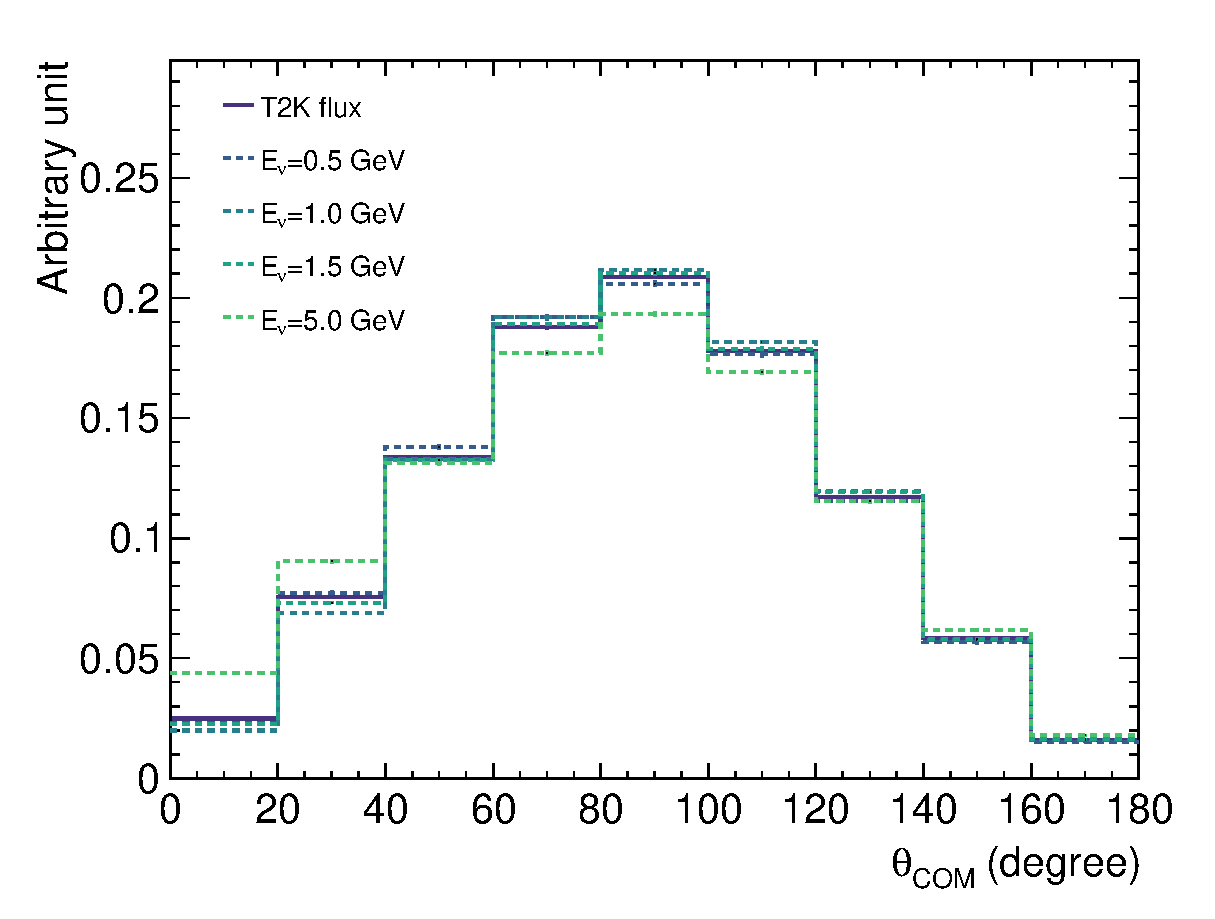
\includegraphics[width=\textwidth]{figures/COM/anorm-monoEnu-less-flux_da_tan.eps}
          \caption{$\numuccopiop$}
          \label{subfig:enu-comp-cc1pi1p}
     \end{subfigure}
     \begin{subfigure}[ht!]{\dbfigwid\textwidth}
          \centering
          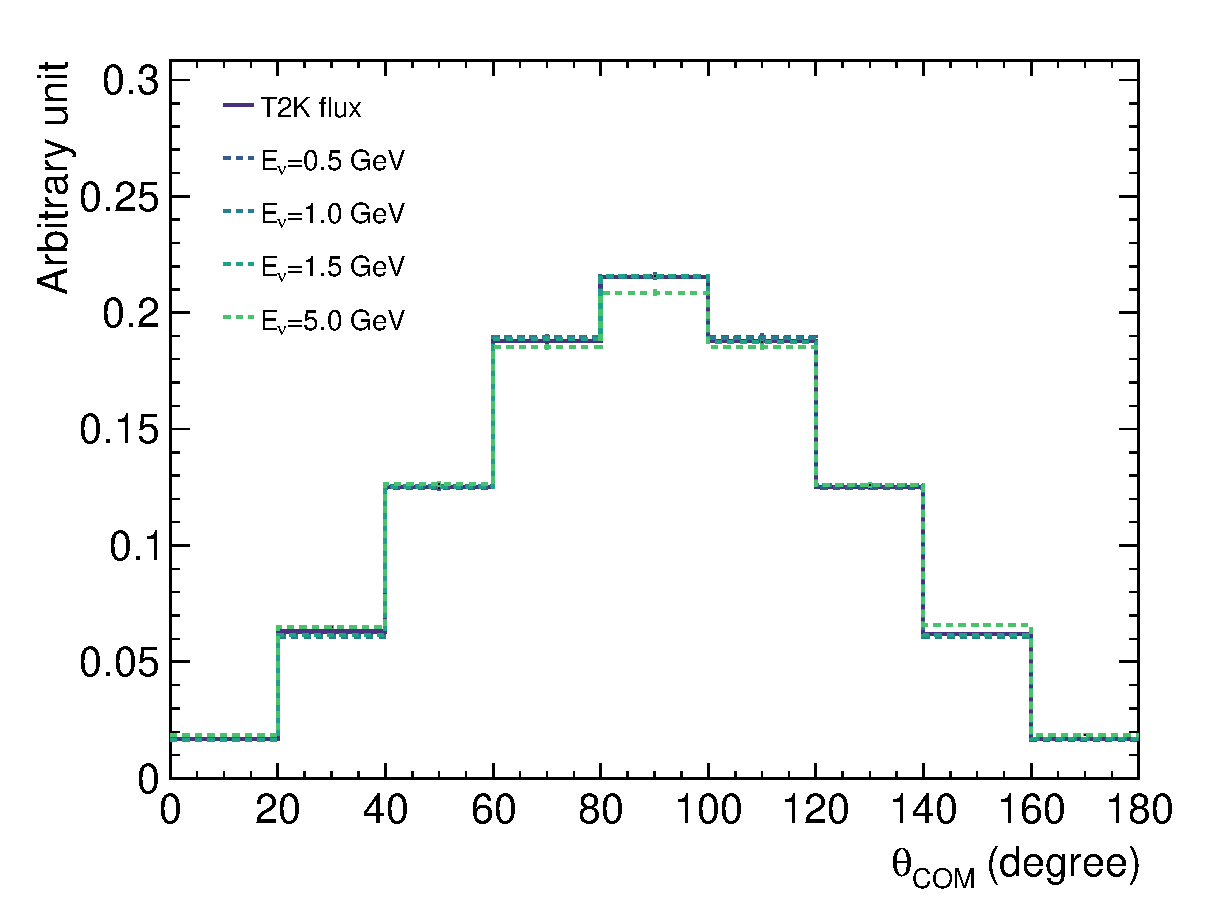
\includegraphics[width=\textwidth]{figures/COM/anorm-monoEnu-less-flux-mode11-_da_tan.eps}
          \caption{$\deltapp$ decay}
          \label{subfig:enu-comp-dpp}
     \end{subfigure}
     \caption{Area normalized comparisons for different $\enu$ fluxes for $\thetacom$.}
     \label{fig:enu-comp}
     \end{figure}

     Besides $\enu$, another important component in the production of resonances is the part of the $\nu$-N interaction modeling that describes the resonance interaction. 
     While $\thetacom$ for a single resonance is largely independent of how the resonance is produced unless there is a strong correlation bewtween the production and decay of the resonance, $\thetacom$ will be affected by the composition of different resonances in the production process. 
     As different resonances can have different decay angular distributions and $\thetacom$ does not distinguish between resonances that have the same decay channel, different combinations of resonances in production modelling will change the $\thetacom$ distribution. 
     As a proxy to investigate the impact of a change in the resonance production model, the axial mass parameter, $\MA$, was varied to an exaggerated and most likely unphysical extent and the effect is shown in Fig.~\ref{fig:ma-comp}. 
     As anticipated, Fig.~\ref{subfig:ma-comp-xsec} demonstrates that varying $\MA$ alters the cross-section.
     However, it is reassuring to observe that the shape of $\thetacom$ remains almost identical, as shown in Fig.~\ref{subfig:ma-comp-area}. 

     \begin{figure}
     \centering
     \begin{subfigure}[b]{\dbfigwid\textwidth}
          \centering
          \includegraphics[width=\textwidth]{figures/COM/xnorm-ma_da_tan.eps}
          \caption{cross section normalized}
          \label{subfig:ma-comp-xsec}
     \end{subfigure}
     \begin{subfigure}[b]{\dbfigwid\textwidth}
          \centering
          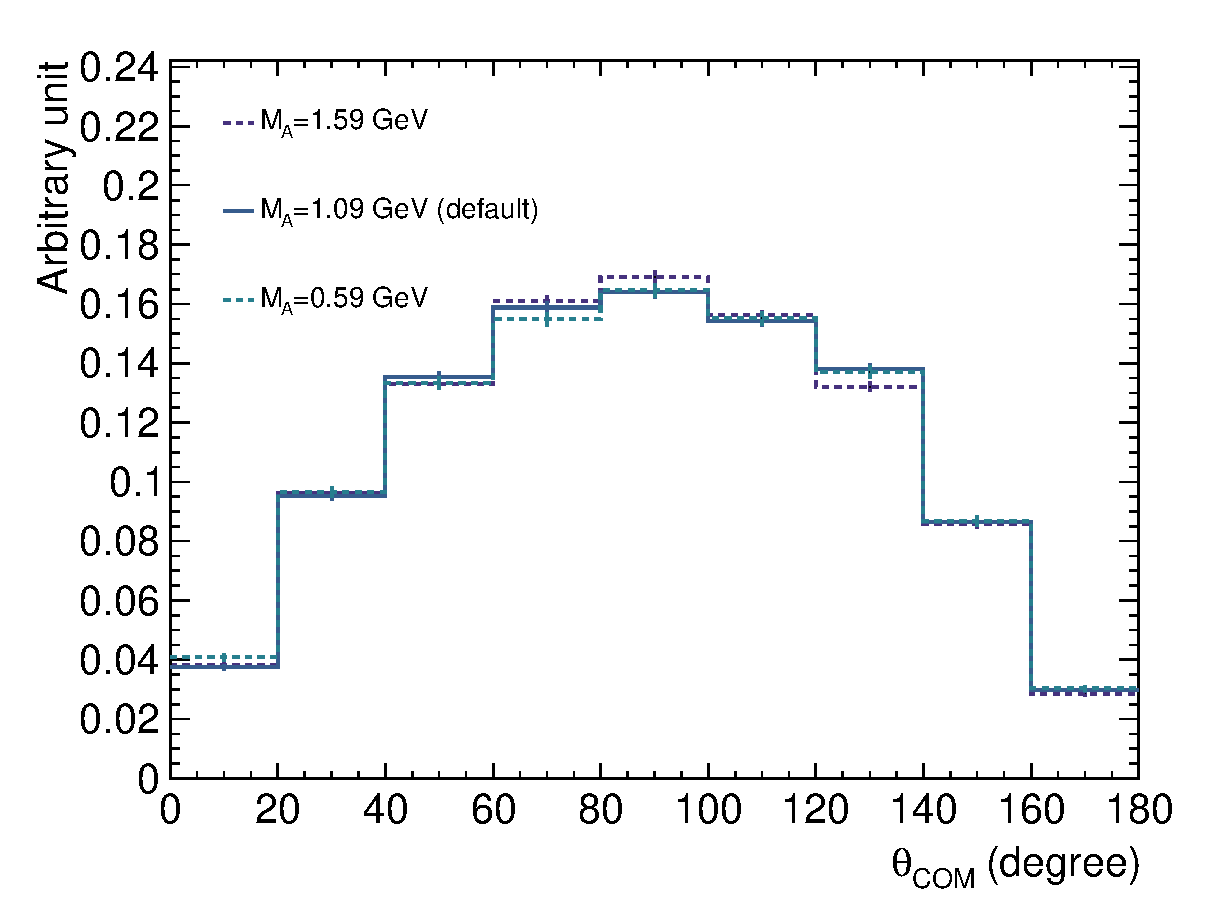
\includegraphics[width=\textwidth]{figures/COM/anorm-ma_da_tan.eps}
          \caption{area normalized}
          \label{subfig:ma-comp-area}
     \end{subfigure}
     \caption{Comparisons for different $\MA$ values with T2K flux. }
     \label{fig:ma-comp}
     \end{figure}


     \subsection{Discussion}
     \label{sec:dis}
     The above simulation studies demonstrate that the COM angle is a novel variable with several advantages, and its measurement will be valuable for studying FSI independently of IS.

     Although the analysis focus of $\thetacom$ is on nuclear effects, it is inherently affected by the resonance interaction modelling. 
     Fortunately, the $\nu$-N interaction is relatively well-understood, particularly through direct studies of $\nu$-H interactions. 
     As a result, future RES modeling is not expected to deviate drastically from current predictions, which are constrained by bubble chamber data.
     Even if the RES model were to change significantly, as explored in Fig.~\ref{fig:ma-comp}, the impact on the shape of $\thetacom$ remains minimal, particularly for the T2K flux.
     This suggests that FSI models tuned using $\thetacom$, e.g. following the methodology in Ref.~\cite{GENIE:2021zuu}, will continue to be applicable even if the RES model undergoes future updates, thereby enhancing the robustness of such FSI model tuning.

     As noted in Sec.~\ref{sec:com}, the $\thetacom$ distribution is influenced by the production of higher resonances that decay through the same channels as $\deltapp$.
     The impact is two-fold.
     Firstly, due to general difference of $\thetaR$ from $\thetapidel$, $\thetacom$ would start to deviate from $\thetapidel$ (smeared by FSI), as shown in Fig.~\ref{subfig:enu-comp-cc1pi1p}. 
     Although $\thetacom$ is inspired by $\thetapidel$, it is not restricted to the reconstruction or estimation of $\thetapidel$. 
     Rather, $\thetacom$ by definition is the superposition of all energetically accessible $\thetaR$, with $\thetapidel$ being the dominant component at low energy.
     If all $\thetaR$'s are relatively well understood, a simple theoretically motivated expectation of $\thetacom$ can be obtained by adding the contributions from all possible R according to the relative production ratios.
     This simple approach is complicated by the second point - even with a complete understanding of the FSI model, the predicted $\thetacom$ distribution would deviate from measurements due to correlations among different resonance production modes, i.e. the overall $\thetacom$ is not simply a linear combination of the individual $\thetaR$ contributions.
     Nevertheless, the influence of higher resonances is minor for low-energy neutrino beams and can be further reduced by applying an upper cut on the COM total energy, ensuring that the selected events predominantly arise from $\deltapp$ decay.
     As FSI modeling improves and single-resonance models are refined through constraints from other experiments, the COM total energy cut could be lifted. 
     This would enable the full $\thetacom$ distribution to be used for studying correlations and advancing RES modeling.

     The sensitivity of the COM frame to FSI can be leveraged not only to study FSI but also to select events without FSI. 
     These events are primarily composed of $\nu$-H interactions, which provide a unique opportunity for precise measurements of the axial current—a feature specific to neutrinos. 
     Additionally, a $\nu$-H sample allows for the improvement of $\nu$-H modeling without the complications of IS and FSI, facilitating accurate neutrino energy reconstruction. 
     These advantages have driven significant efforts to develop techniques for selecting a high-purity $\nu$-H sample, as seen in Ref.~\cite{Lu:2015hea,MINERvA:2023avz,Baudis:2023tma}.
     While Ref.~\cite{Baudis:2023tma} and Ref.~\cite{MINERvA:2023avz} focuses on neutrino and antineutrino pion-less events respectively, Ref.~\cite{Lu:2015hea} applies to the same event topology as the COM total energy. 
     Preliminary studies have shown that applying a cut on COM energy can remove events with minimal transverse momentum imbalance, which could be combined with cuts on $\dptt$ and $\dpt$ to create a high-purity $\nu$-H sample. 
     This approach will be explored further in future studies.

     Although the COM angle shares a similar reconstruction target with the Adler angle, there are key differences, as discussed in Sec.~\ref{sec:ana}. 
     While these differences may appear minor, the conceptual distinction makes tuning the FSI model using the COM angle more adaptable to future developments. 
     Furthermore, the analyses presented here are based on true information without any realistic fluctuations, meaning that challenges related to reconstruction—particularly those involving neutrino energy for the Adler angle—are not considered. 
     Therefore, the full potential of the COM angle will be better realized in a cross-section measurement that accounts for these complexities.

     \subsection{Conclusion}
     This study introduces a novel set of variables—the COM angle and total energy.
     These variables offer several advantageous properties, motivating their use in future cross-section measurements.
     These measurements have the potential to significantly improve our understanding and modeling of FSI processes in neutrino-nucleus interactions, thereby contributing to more accurate neutrino cross-section predictions.

\section{Hydrogen Sample Selection}
\label{sec:mc-hydrogen}
The importance of a high-purity $\nu$-H sample has been discussed in Sec.~\ref{sec:dis} (check where exactly).
There has been growing interest and efforts in developing techniques to select such a sample, as seen in Ref.~\cite{Lu:2015hea,MINERvA:2023avz,Baudis:2023tma}.
While Ref.~\cite{MINERvA:2023avz} and Ref.~\ref{Baudis:2023tma} select $\nu$-H events in the antineutrino and neutrino pion-less samples respectively, Ref.~\cite{Lu:2015hea} applies to events with pions in the final state. 
They serve as good complements to each other.
The proposition in Rec.~\cite{Lu:2015} is to use $\dptt$ to select $\nu$-H events.
It is difficult to achieve optimal efficiency and purity with a one-dimensional cut. 
Hence, the COM total energy cut is proposed as a complementary cut to $\dptt$, and this section shall demonstrate its effectiveness.

\subsection{MC Study}
\label{sec:mc-hydrogen-ana}
     The key to remove carbon backgrounds from the hydrogen events is to identify the variables that can effectively distinguish between the two.
     Hence, distributions decomposed according to the type of the target nucleus are shown in Fig.~\ref{fig:hsel-tki-decomp} for the proposed variables.

     As shown in Fig.~\ref{subfig:hsel-dptt-stack}
     \begin{figure}
     \begin{subfigure}[b]{\dbfigwid\textwidth}
          \centering
          \includegraphics[width=\textwidth]{figures/perf/tki/SFGpTPCmu_dptt_stack_al15.eps}
          \caption{$\dptt$}
          \label{subfig:hsel-dptt-stack}
     \end{subfigure}
     \begin{subfigure}[b]{\dbfigwid\textwidth}
          \centering
          \includegraphics[width=\textwidth]{figures/perf/tki/SFGpTPCmu_dpt_stack_al15.eps}
          \caption{$\dpt$}
          \label{subfig:hsel-dpt-stack}
     \end{subfigure}
     \caption{Decomposed distributions for $\dptt$ and $\dpt$ for hydrogen and carbon events.}
     \label{fig:hsel-tki-decomp}
     \end{figure}
     Based on $\dptt$ alone, the most effective cut will be to have $-10\mevc \leq \dptt \leq 30\mevc$.
     This cut leads to a sample of $16$ hydrogen events and $16$ carbon events, with a purity of $50\%$.
     In comparison, Ref.~\cite{MINERvA:2023avz} observed ``5,580(180) signal events over the estimated background of 12,500 events'', the purity of which is considerably lower than the $50\%$ achieved here, but the total number of events is much higher.
     Hence, for the T2K sample to be most useful, the purity needs to be as high as possible so as to reduce the systematic uncertainties for any parameter measurements.

     As SFGD is excellent in 3D tracking, a cut on $\dpt$ might further help reduce carbon backgrounds.
     A similar decomposition is shown in Fig.~\ref{subfig:hsel-dpt-stack} for $\dpt$.
     It is observed that both the $\dpt$ and $\dptt$ for hydrogen events centre around $0$, while the carbon events are much more spread out.
     As the two variables are not completely independent, as $\abs{\dptt} \leq \dpt$, it is easier to identify the appropriate two dimensional cut by plotting the two variables together, as shown in Fig.~\ref{fig:hsel-dpt-dptt} for hydrogen and carbon separately.
     \begin{figure}
          \begin{subfigure}[b]{\dbfigwid\textwidth}
               \centering
               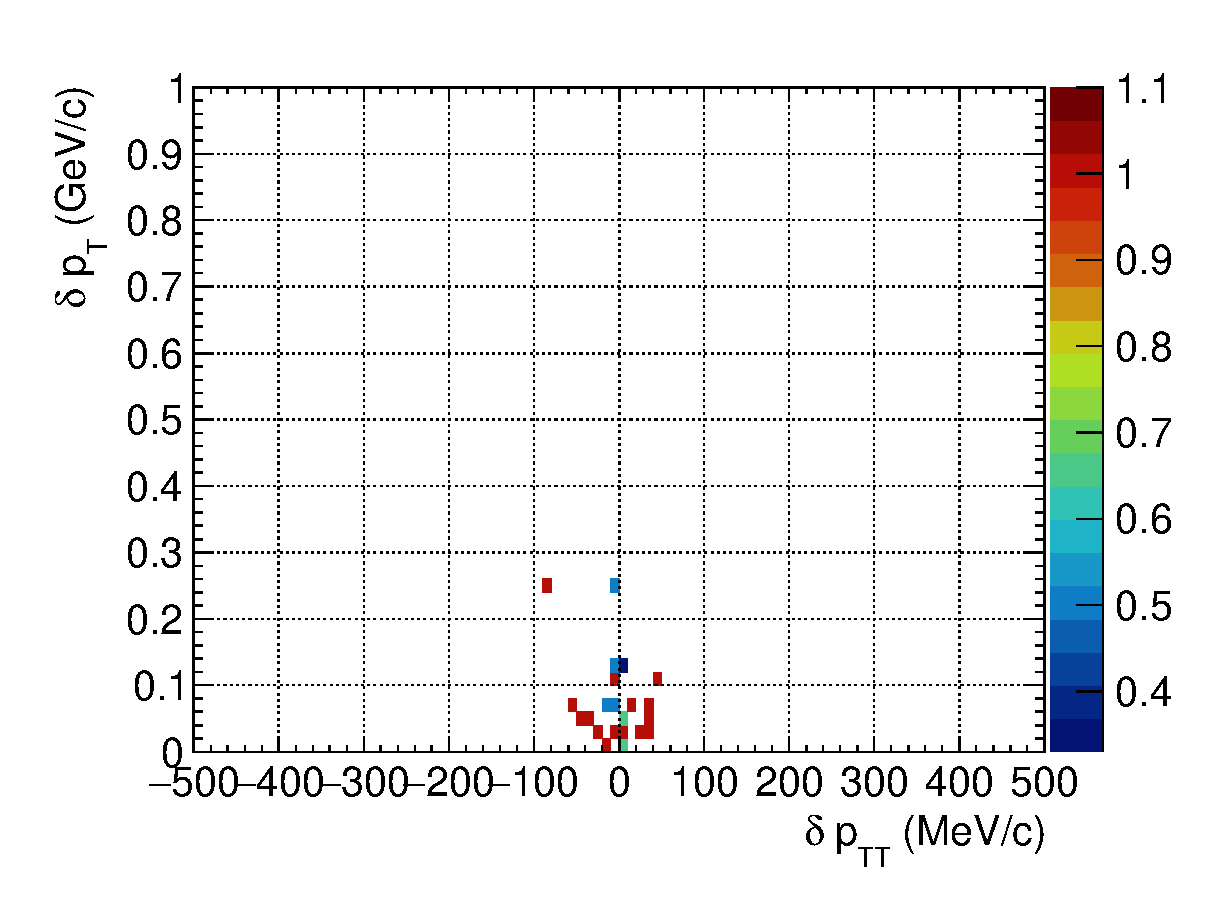
\includegraphics[width=\textwidth]{figures/perf/tki/SFGpTPCmu_dptt_colnor_vs_dpt_hist2d_al15_H.eps}
               \caption{Hydrogen events}
               \label{subfig:hsel-dpt-dptt-h}
          \end{subfigure}
          \begin{subfigure}[b]{\dbfigwid\textwidth}
               \centering
               \includegraphics[width=\textwidth]{figures/perf/tki/SFGpTPCmu_dptt_colnor_vs_dpt_hist2d_al15_C.eps}
               \caption{Carbon events}
               \label{subfig:hsel-dpt-dptt-c}
          \end{subfigure}
          \caption{Two-dimensional distributions of $\dpt$ and $\dptt$ for hydrogen and carbon events.}
          \label{fig:hsel-dpt-dptt}
     \end{figure}
     Fig.~\ref{fig:hsel-dpt-dptt} suggests the cuts, $\dpt < 80\mevc$ and $-40\mevc \leq \dptt \leq 30\mevc$, which leads to a sample of $19$ hydrogen events and $10$ carbon event, with a purity of $65.5\%$.
     This is the optimal purity and efficiency achievable by using TKI variables only.
     To further improve the purity, additional cut on the COM variables is proposed.
     Similar to Fig.~\ref{fig:hsel-tki-decomp}, the decompositions for the COM variables are shown in Fig.~\ref{fig:hsel-com-decomp}.
     Although FSI alters the $\thetacom$ distributions, leading to distinct distributions between hydrogen and carbon, but as $\thetacom$ for hydrogen is expected to be uniform across the entire range, the cut on $\thetacom$ to select hyrodgen is not expected to be effective.
     Note that to show the wide range of $\thetacom$ for hydrogen, the colours for hydrogen and carbon are switched in Fig.~\ref{subfig:hsel-com-theta} respect to others.
     In contrast, without FSI, $\ecom$ is expected to centre around the mass of the resonance, which is $1232\mev$ for $\deltapp$, while the carbon events are expected to have a much wider distribution as shown in Fig.~\ref{subfig:hsel-com-edelta}.
     \begin{figure}
     \begin{subfigure}[b]{\dbfigwid\textwidth}
          \centering
          \includegraphics[width=\textwidth]{figures/perf/tki/SFGpTPCmu_edelta_stack_al14.eps}
          \caption{$\ecom$}
          \label{subfig:hsel-com-edelta}
     \end{subfigure}
     \begin{subfigure}[b]{\dbfigwid\textwidth}
          \centering
          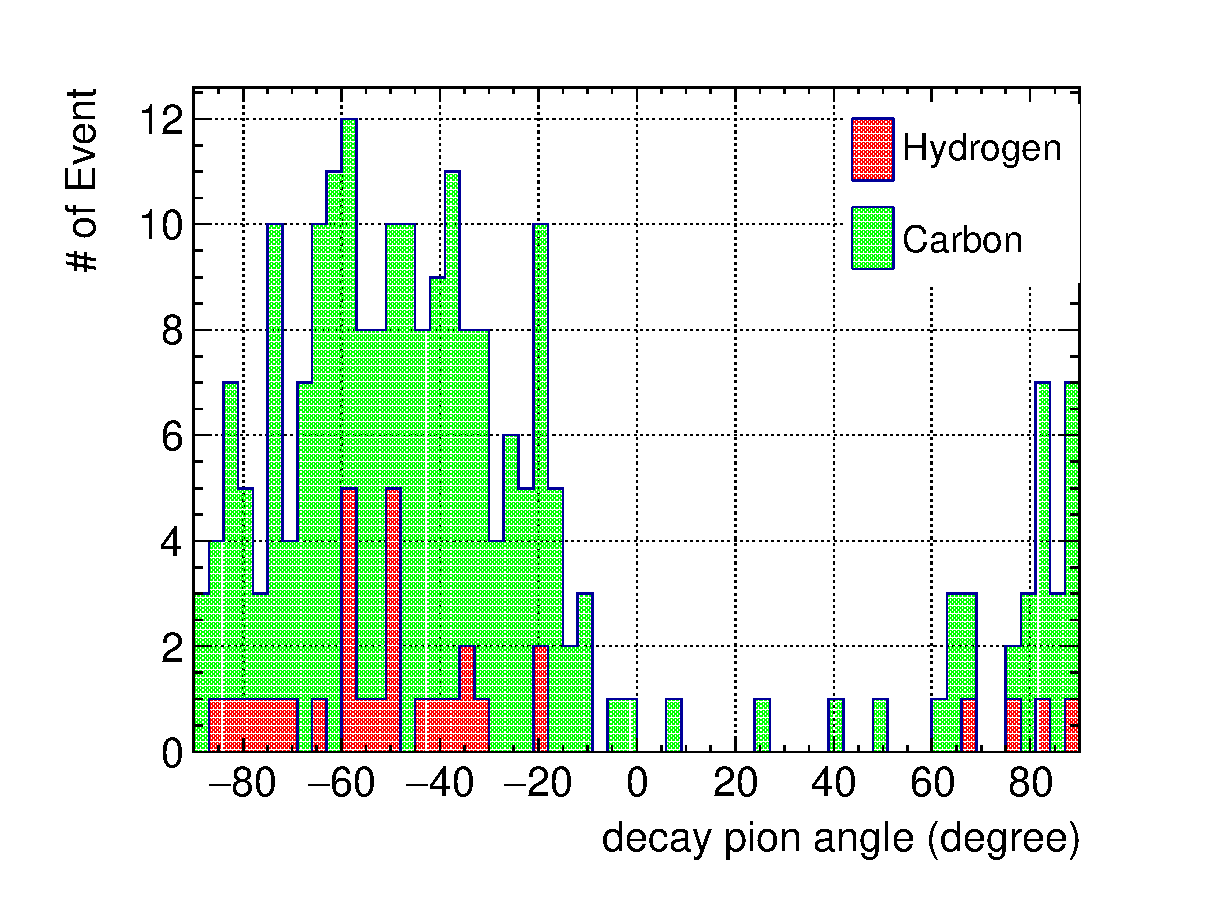
\includegraphics[width=\textwidth]{figures/perf/tki/SFGpTPCmu_dang_stack_al15.eps}
          \caption{$\thetacom$}
          \label{subfig:hsel-com-theta}
     \end{subfigure}
     \caption{Decomposed distributions for $\ecom$ and $\thetacom$ for hydrogen and carbon events.}
     \label{fig:hsel-com-decomp}
     \end{figure}
     Hence, an additional cut, $???<\ecom<???$, is implemented to further reduce the carbon backgrounds, achieving a sample of $18$ hydrogen events and $5$ carbon events, with an impressive purity of $78\%$.

     To demonstrate the effectiveness of these cuts, the $\dptt$ distributions are plotted step-wise in Fig.~\ref{fig:hsel-dptt-step}.
     Comparing the $\dptt$ distributions before and after each cut, namely the cuts on $\dpt$ and $\ecom$, it is evident that these cuts successfully remove carbon backgrounds in the low $\dptt$ region, which is impossible to remove based on $\dptt$ alone.
     Furthermore, by comparing, Fig.~\ref{subfig:} and Fig.~\ref{subfig:}, it is demonstrated that the cut on $\ecom$ is capable of removing carbon backgrounds that cannot be removed by the transverse variables.
     Hence, all three variables are indispensable for achieving the optimal purity and efficiency.
     \begin{figure}
     \begin{subfigure}[b]{\trfigwid\textwidth}
          \centering
          \includegraphics[width=\textwidth]{figures/perf/tki/SFGpTPCmu_dptt_stack_al15.eps}
          \caption{No cut}
          \label{subfig:hsel-dang-nocut}
     \end{subfigure}
     \begin{subfigure}[b]{\trfigwid\textwidth}
          \centering
          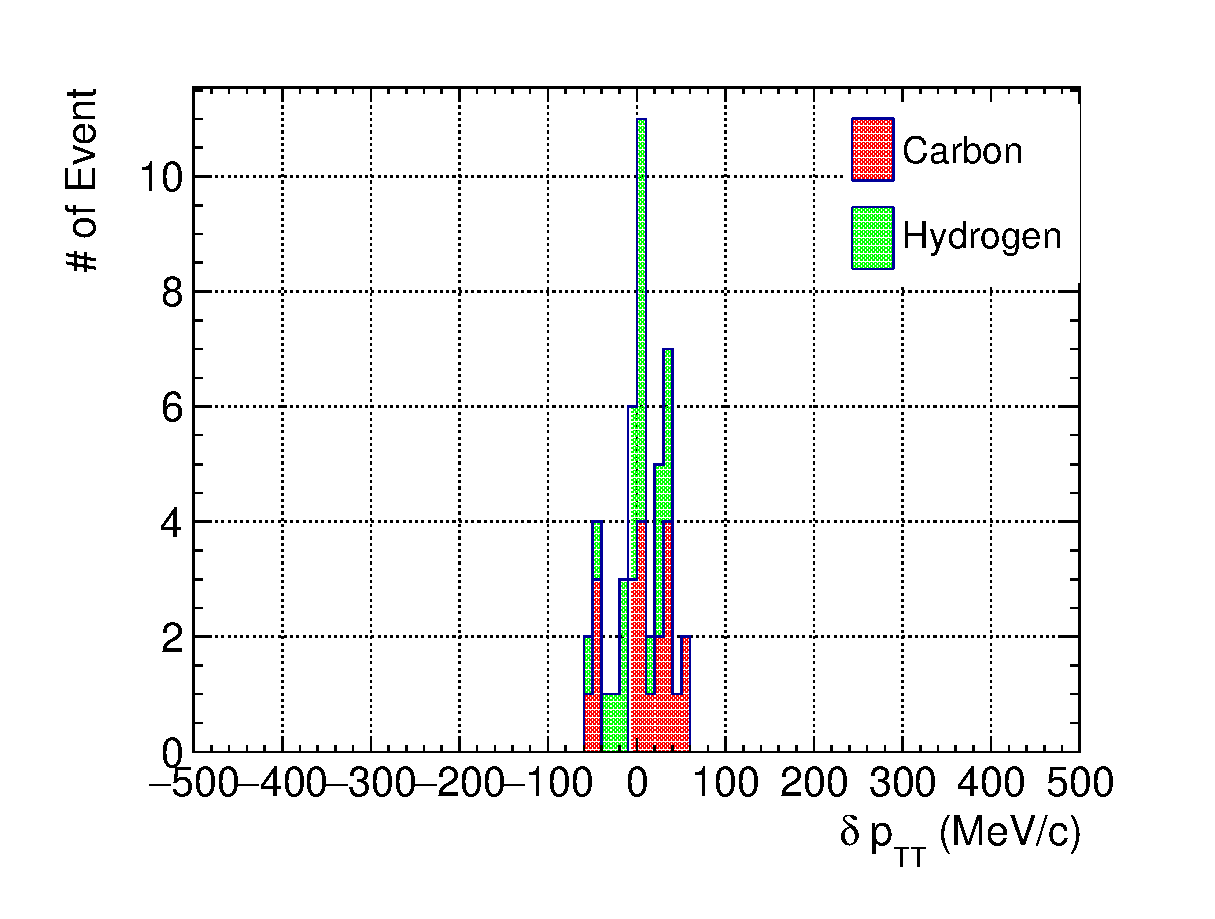
\includegraphics[width=\textwidth]{figures/perf/tki/SFGpTPCmu_dptt_stack_al15_dpt80.eps}
          \caption{$\dpt < 80\mevc$}
          \label{subfig:hsel-dang-dpt80}
     \end{subfigure}
     \begin{subfigure}[b]{\trfigwid\textwidth}
          \centering
          \includegraphics[width=\textwidth]{figures/perf/tki/SFGpTPCmu_dptt_stack_al15_GetH_dpt80_wdang.eps}
          \caption{$\dpt < 80\mevc$ and $\ecom$ cut}
          \label{subfig:hsel-dang-dpt80-ecom}
     \end{subfigure}
     \caption{Step-wise $\dptt$ distributions for hydrogen and carbon events.}
     \label{fig:hsel-dptt-step}
     \end{figure}

     \subsection{Discussion}
     Due to the limited amount of MC events available and the relatively small fraction of resonance event in the T2K beam, the statistics of the selection is too small to be conclusion.
     However, the results presented here are promising and suffice in demonstrating the efficacy of using $\ecom$ to remove carbon backgrounds that could not be removed with the transverse variables.

   

     
     